\chapter{Investimento residencial e bolha de ativos em um modelo SFC com supermultiplicador sraffiano}\label{CapModelo}
%TODO: Alterar título

%\epigraph{[I]f you are a true simplifier and not just
%sloppy and lazy then you must be able to claim to arrive at essentials which are also to be
%found in what you regard as complicated}{Frank Hahn}

O presente capítulo é o ponto de chegada desta pesquisa em que são reunidos os esforços dos capítulos anteriores. Enquanto o capítulo primeiro elegeu o supermultiplicador sraffiano como o modelo teórico a ser adotado, o capítulo seguinte  enfatizou o papel do investimento residencial para a dinâmica macroeconômica destacando a taxa própria de juros do imóveis como determinante de sua taxa de crescimento para caso norte-americano. Desse modo, cabe a este capítulo construir o modelo teórico por meio da metodologia \textit{Stock-Flow Consistent}  que seja útil para ajudar a explicar alguns dos fatos estilizados da economia norte-americana do período de 1992 a 2019, como visto no capítulo anterior.

A razão do porquê da escolha desta metodologia decorre do tratamento adequado das relações financeiras, enriquecendo o modelo do supermultiplicador sraffiano tal como em \textcite{brochier_supermultiplier_2018}. Antes de avançar, cabe destacar que se optou pelo modelo mais parcimonioso possível de modo que apenas os setores estritamente necessários foram incluídos. Sendo assim, será simulado um modelo em que as famílias capitalistas passam a investir em imóveis e, assim, a economia passa a ter dois estoques de capital distintos: imóveis e das firmas. Para tanto, o investimento residencial é financiado por meio das hipotecas que são ofertadas sem restrições. 
Além disso, o mercado imobiliário pode ser considerado insensível a competição externa --- como em \textcite{duesenberry_investment_1958} --- de modo que essa separabilidade permite simplificar ao caso de uma economia fechada.

%TODO Rever separabilidade e hipótese de economia fechada.

Dito isso, a seção \ref{IntroSFC} irá expor a metodologia utilizada enquanto a seção \ref{SecModelo} apresenta o modelo. Com as equações em mãos, é exposta a solução analítica (sec. \ref{SecAnalitica}) e serão analisados os impactos na dinâmica macroeconômica de mudanças na distribuição de renda, na taxa de juros, na inflação imobiliária e no componente autônomo da taxa de crescimento do investimento residencial (sec. \ref{SecChoques}). Com isso, espera-se avaliar a dinâmica entre os dois estoques de capital existentes.
Por fim, são apresentadas as conclusões do modelo.

\section{Metodologia SFC: Uma breve introdução}
\label{IntroSFC}


A presente seção ter por objetivo apresentar as etapas e procedimentos da metodologia \textit{Stock Flow Consistent} (adiante SFC\footnote{Cabe aqui destacar que tal nomenclatura decorre do trabalho de \textcite{dos_santos_keynesian_2006}.})\footnote{Para uma análise mais pormenorizada das linhagens da abordagem SFC, ver \textcite{caverzasi_stock-flow_2013}.}. De forma bastante sucinta, tal metodologia é composta de três procedimentos: (i) determinação da estrutura contábil; (ii) exposição das equações comportamentais e; (iii) solução. Dito isso, a figura \ref{Resuminho} pretende resumir as etapas mencionadas e explicitar a diferença entre a \textit{metodologia} SFC um \textit{modelo} SFC. 

\begin{figure}[htb]
	\caption{Resumo esquemático da Metodologia SFC}
	\label{Resuminho}
	\centering
	\begin{tikzpicture}
	[node distance = 1cm, auto,font=\footnotesize,
	% STYLES
	every node/.style={node distance=3cm},
	% The comment style is used to describe the characteristics of each force
	comment/.style={rectangle, inner sep= 5pt, text width=4cm, node distance=0.25cm, font=\scriptsize\sffamily},
	% The force style is used to draw the forces' name
	force/.style={rectangle, draw, fill=black!10, inner sep=5pt, text width=4cm, text badly centered, minimum height=1.2cm, font=\bfseries\footnotesize\sffamily}] 
	
	% Draw forces
	\node [force] (rivalry) {Hipóteses};
	\node [force, above of=rivalry, fill=red!70] (substitutes) {Equações comportamentais};
	\node [force, text width=3cm, dashed, left=1.5cm of substitutes,fill=blue!50] (state) {Metodologia SFC};
	\node [force, left=1cm of rivalry] (suppliers) {Estrutura contábil};
	\node [comment, below=0.25 of suppliers] (comment-suppliers) {Relação entre lado real \\e financeiro};
	\node [force, right=1cm of rivalry] (users) {Solução};
	\node [force, right=1cm of substitutes, dashed, fill=purple!50 ] (PK) {Modelo \\SFC};
	%	\node [force, below of=rivalry] (entrants) {Threat of new entrants};
	
	%%%%%%%%%%%%%%%
	% Change data from here
	
	% RIVALRY
	\node [comment, below=0.25 of rivalry] (comment-rivalry) {Cambridge/New Cambridge\\
		Kaleckiano\\
		\textbf{Supermultiplicador Sraffiano}};
	
	
	% SUBSTITUTES
	%\node [comment, right=0.25 of substitutes] {};
	
	% USERS
	\node [comment, below=0.25 of users] {Analítico\\
		\textbf{Simulação}};
	
	% NEW ENTRANTS
	%	\node [comment, right=0.25 of entrants] {(+) EC vs. Microsoft};
	
	% PUBLIC POLICIES
	%	\node [comment, text width=3cm, below=0.25 of state] {(1) Estrutura contábil\\
	%	(2) Equações comportamentais\\
	%	(3) \textit{Closure} do modelo};
	
	%%%%%%%%%%%%%%%%
	
	% Draw the links between forces
	\path[->,thick] 
	(rivalry) edge (substitutes)
	(suppliers) edge (rivalry)
%	(rivalry) edge (users)
	(state) edge (substitutes)
	(state) edge (suppliers)
	(substitutes) edge (PK)
	(PK) edge (users);
	
	%(entrants) edge (comment-rivalry);
	
	\end{tikzpicture} 
	\caption*{Fonte: \textcite[p.~64, adaptado]{da_silveira_politica_2017}}

	
\end{figure}


As etapas contábeis da abordagem SFC constituem em\footnote{Esta seção não pretende expor a metodologia pormenorizadamente, mas sim expor seus procedimentos de modo a esclarecer as etapas que foram adotadas. Dito isso, a construção das matrizes a serem usadas fica a cargo da seção \ref{SecModelo}. Para uma apresentação mais gradual, ver \textcite[Capítulo 4]{da_silveira_politica_2017}.}: (i) seleção dos setores institucionais e dos ativos a serem incorporados; (ii) mapeamento das relações dos fluxos entre os mencionados setores por meio da construção da matriz de fluxos; (iii) construção da matriz dos estoques de riqueza (real e financeira) em que são contabilizadas os ativos e passivos  bem como a posição líquida de cada setor; (iv) identificação das formas que os fluxos são financiados e sua respectiva acumulação nos estoques. Desse modo, o rigor contábil adotado faz com que o grau de liberdade, ou seja arbitrariedade, do modelo diminua. Como todo modelo macroeconômico, ao partir de um aparato analítico baseado em identidades contábeis, surgem restrições que precisam ser seguidas mas o que distingue a metodologia SFC das demais é a conexão do lado real com o financeiro de forma integrada.

Vale destacar que as identidades contábeis são o ponto de partida, mas não são suficientes para garantir a consistência do modelo\footnote{Exemplo disso pode ser visto na exposição de  \textcite[p.~27--8]{godley_monetary_2007}  a despeito da contabilização das ações que não são, legalmente, um passivo das firmas e, portanto, o pagamento de dividendos não é uma obrigação contratual. Apesar disso, considera-se que as ações emitidas pelas firmas são similares aos \textit{corporate bonds}, garantindo a consistência do modelo. O que pretende ser destacado é que por mais que tal simplificação seja razoável, não deixa de ser uma hipótese.}. Para isso, é necessário que a soma da posição financeira líquida dos setores institucionais seja zero de modo que não existam ``buracos negros''. Tal procedimento garante que para que um setor acumule riqueza financeira, outro precisa necessariamente liquidá-la. Isto posto, conclui-se a exposição da estrutura contábil da metodologia SFC a partir das identidades macroeconômicas. 

Por mais que esta etapa é centrada na contabilidade social, isso não implica que não possua um componente teórico associado. A título de exemplo, \textcite[p.~15--16]{macedo_e_silva_peering_2011}  pontuam que estão presentes elementos pós-keynesianos: (i) os agentes econômicos são categorizados de acordo com o tipo de estoque de riqueza que possuem; (ii) os agentes celebram contratos que impactam sua riqueza e geram fluxos monetários que implicam novas mudanças na composição patrimonial desses agentes; (iii) ganhos e perdas de capital afetam o valor dos estoques que impactam na dinâmica do sistema; (iv) a composição patrimonial dos agentes e setores evolui de forma assimétrica de acordo com o grau de alavancagem, preferência
pela liquidez/risco e (v) o acúmulo de ativos e passivos pelos agentes interfere na correlação de forças da economia. 

Desse modo, por mais que a estrutura contábil parta das identidades, isso não a isenta de teoria. No entanto, por se tratar de identidades, nada de causal pode ser extraído delas. As relações de causalidade do modelo (agora modelo e não metodologia) decorrem das equações comportamentais que, respeitando a consistência, podem ser de qualquer linhagem teórica (\textit{e.g.} kaleckiana, sraffinana, neoclássica, etc.). A ênfase em tratar a abordagem SFC enquanto uma metodologia decorre da flexibilidade de incluir inúmeras teorias e propostas apesar da rigidez de seus procedimentos. Apenas para elencar (e não esgotar) alguns temas caros a heterodoxia, tal abordagem permite tratar as formas de financiamento das firmas \cites{asimakopulos_kalecki_1983}{skott_finance_1988}{messori_financing_1991}; endogeneidade da moeda e importância do sistema bancário \cites{messori_financing_1991}{dow_horizontalism:_1996}{arestis_theoretical_1996}{godley_money_1999}{lavoie_note_1999}{lima_macrodynamics_2007}; endividamento, distribuição de renda e financeirização \cites{palley_inside_1996}{wolfson_irving_1996}{palley_money_1997}{palley_financial_2002}{dos_santos_revisiting_2009}{palley_inside_2010}{hein_finance-dominated_2012} e, apenas para restringir os temas; análises empíricas e proposições de política econômica \cites{godley_seven_1999}{godley_fiscal_2007}{godley_simple_2007}{arestis_income_2011}{zezza_design_2019}. 

A mesma variabilidade de temas passíveis de serem abordados pela metodologia SFC se estende para a pluralidade dos ativos e do grau de complexidade financeira de cada modelo. Uma forma de visualizar tal flexibilidade é por meio da figura \ref{Heatmap} em que são mapeados os ativos mais frequentes. No entanto, este gráfico também revela que a literatura não dá a devida atenção ao investimento residencial\footnote{Deve ser pontuada a notória exceção de \textcite{zezza_u.s._2008} em que é apresentado um modelo com imóveis em um aparato kaleckiano mas não trata de questões envolvendo ganhos de capital ou dos determinantes do investimento residencial.}, sendo o ativo menos estudado. 
\begin{figure}
    \centering
    \caption{Mapa de calor dos ativos modelados com SFC}
    \label{Heatmap}
    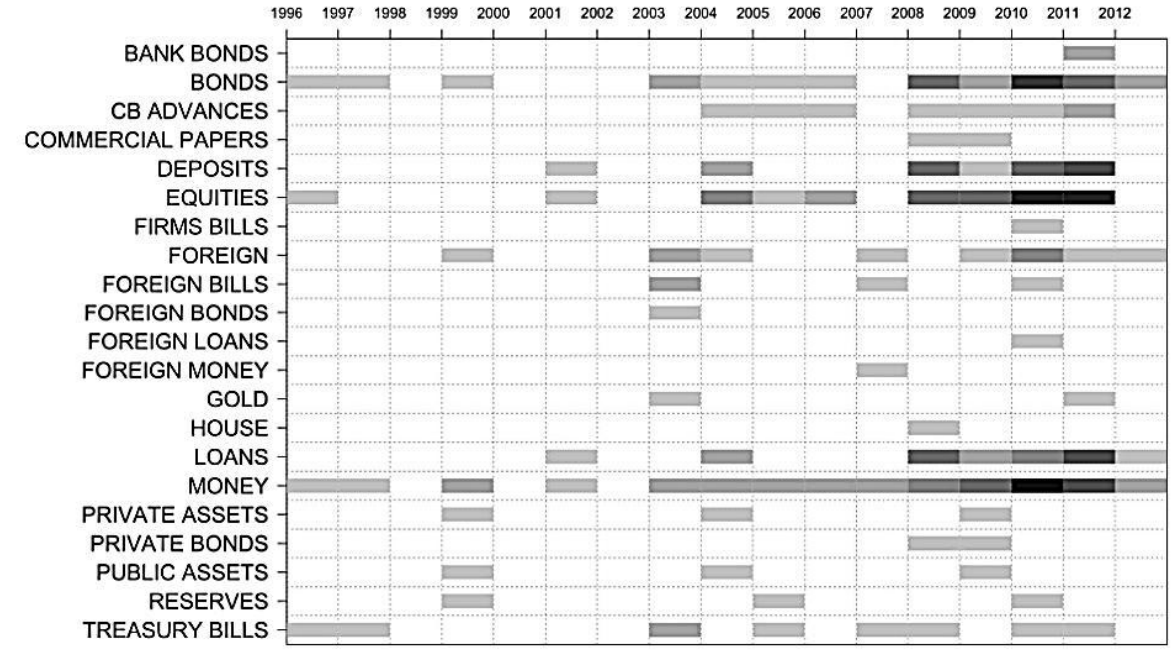
\includegraphics[width = 0.9\textwidth]{Modelo/Caverzassi_Heatmap.png}
    \caption*{\textbf{Fonte:} \textcite[p.~4]{caverzasi_stock-flow_2013}}
\end{figure}


%BREVE REVISÃO MODELOS SHIPMAN + GRÁFICO CAVERZASSI



Feitas essas ressalvas, dada a estrutura contábil e explicitadas as hipóteses (via equações comportamentais), resta seguir para a solução do modelo. Como pontuam \textcite{caverzasi_stock-flow_2013}, existem duas vias: (i) simulação e (ii) discursiva. A primeira delas permite expor de forma mais clara as relações entre as variáveis de modelos mais complexos em que a solução analítica não é facilmente encontrada. No entanto, tal caminho fez com que o grau de complexidade dos modelos simulados fosse exponencializada de modo que a intuição econômica torna-se facilmente turva. Diante destas complicações, o presente capítulo prioriza a parcimônia de modo que serão incluídos apenas os elementos necessários para a narrativa. A justificativa deste procedimento decorre da maior clareza que tal modelagem frente a um menor ``realismo''. Além disso, tal postura permite encontrar soluções analíticas com maior facilidade de modo que são explicitados os parâmetros mais relevantes para as trajetórias de longo prazo. 
Apesar de parcimoniosidade do modelo, a simulação tem a vantagem de fornecer informações que não se restringem às soluções de equilíbrio e que vão além de um sistema de equações em que é possível visualizar as relações entre algumas variáveis de interesse. 
Dito isso, a seção seguinte expõe o modelo que será simulado adiante.
\section{Modelo}
\label{SecModelo}

Por padrão, as variáveis exógenas, $j$ diga-se, serão indicadas por $\overline{j}$ enquanto os parâmetros serão denotados por letras gregas. Além disso, as equações não numeradas são apenas etapas algébricas enquanto as numeradas estão presentes nas rotinas utilizadas. Por fim, vale a menção de que os códigos deste modelo estão disponíveis e foram escritos em \textit{python} com o uso do pacote \textit{pysolve3} que foi desenvolvido ao longo desta pesquisa.

\paragraph*{Equações gerais}
O produto é determinado pelo estoque de capital criador de capacidade assim como pelo trabalho homogêneo. Além disso, supõe-se temporariamente que não estão presentes inflação de bens bem como depreciação\footnote{A ausência de depreciação é meramente simplificadora e será incluída nas versões futuras deste modelo. Vale mencionar que um dos objetivos desta pesquisa é incorporar e analisar os impactos da inflação de ativos.}.  Diferentemente de \textcite{nikiforos_utilization_2016} e \textcite{dutt_observations_2018}, supõe-se que estão ausentes retornos crescentes de escala e progresso tecnológico.

Por se tratar de uma economia sem relações externas e sem governo, o produto determinado pelos componentes da demanda ($Y$) é a soma do consumo ($C$) e investimento das famílias ($Ih$) e das firmas ($If$) em que apenas este último é criador de capacidade produtiva ao setor privado:

\begin{equation}
\label{_Y}
    Y = [C + Ih] + [If]
\end{equation}
da equação acima é possível deduzir o investimento total ($It$):

\begin{equation}
\label{_It}
    It = If + Ih
\end{equation}

Considerando uma função de produção \textit{à la} leontieff, o produto potencial ($Y_{FC}$) é determinado por:

$$
Y_{FC} = \min (Y_K, Y_L)
$$
em que $Y_K$ e $Y_L$ são respectivamente produto de plena capacidade e de pleno emprego definidos por:

$$
Y_K = \frac{1}{\overline v}K_{f_{-1}} \hspace{2.5cm} Y_L = \frac{1}{\overline b}L_{-1}
$$
com $v$ e $b$ sendo relações técnicas e $K_f$ e $L$ indicam respectivamente o estoque de capital criador de capacidade ao setor privado e  o trabalho. Tal como é convencional na literatura, supõe-se que o capital é escasso em relação ao trabalho. Nesses termos, o produto potencial é:

\begin{equation}
\label{_YFC}
    Y_{FC} = Y_K
\end{equation}
o que permite escrever o grau de utilização da capacidade ($u$):

$$
u = \frac{Y}{K_f}\cdot \overline v
$$

\begin{equation}
\label{_u}
    u = \frac{Y}{Y_{FC}}
\end{equation}
cuja forma em termos de crescimento equivale a
\begin{equation}
\label{Aux}
\tag{Aux.}
\dot u = (g - g_K)\cdot u_{t-1}
\end{equation}
em que $g_Y$ e $g_K$ são, respectivamente, a taxa de crescimento da demanda e da capacidade produtiva discutidas no capítulo teórico.


A razão pela qual o capital criador de capacidade se difere do estoque de capital total da economia ($K$) se dá pela inclusão do investimento residencial tão comumente ignorado pela literatura que, como pontuado pelo capítulo anterior, possui implicações importantes para a dinâmica da economia norte americana. Dito isso, o estoque de capital é dado por:

\begin{equation}
\label{_K}
    K = Kf + K_{H}
\end{equation}
em que $K_H$ refere ao acúmulo do investimento residencial. Seja $K_k$ a participação dos imóveis no estoque de capital total da economia:

\begin{equation}
\label{_tau}
K_k = \frac{K_H}{K}    
\end{equation}
é possível representar a equação \ref{_K} de forma alternativa:
$$
K = K_k\cdot K + (1-K_k)\cdot K
$$
que será utilizada para o desenvolvimento da solução analítica.

Neste modelo, tal como na tradição Kalekicana e Sraffiana, a distribuição funcional da renda é exógena. Para não recorrer à hipóteses a respeito da estrutura de mercado bem como da determinação de preços das firmas, impõe-se que:

\begin{equation}
    \omega = \overline{\omega} \Leftrightarrow \pi = 1 - \overline{\omega}
\end{equation}
em que $\omega$ e $\pi$ são respectivamente a participação dos salários e dos lucros na renda. O que permite escrever a massa de salários nos seguintes termos:

$$
\omega = \frac{W}{Y}
$$

\begin{equation}
\label{_W}
    W = \omega\cdot Y
\end{equation}

Por fim, cabe explicitar os ativos financeiros presentes no modelo e como são distribuídos entre os diferentes agentes institucionais. As famílias (denotadas pelo subíndice $h$) acumulam riqueza sob a forma de depósitos à vista ($M$) enquanto contraem empréstimos hipotecários ($MO$) para realizar investimento residencial que, no acumulado, é idêntico ao estoque de imóveis ($K_h$). 
%Além disso, tal como pontuado por \textcite{leamer_housing_2007}, possuem acesso a crédito ($N$) a depender do estoque de riqueza (imóveis neste caso) e é financiado por dívida ($L_h$)
As firmas (denotadas pelo subíndice $f$), por sua vez, financiam o investimento em parte por lucros retidos e o restante por empréstimo ($L_f$). Os bancos, portanto, criam crédito (\textit{ex nihilo}) para então recolher os depósitos, todos remunerados pelas respectivas taxas de juros. Com isso, é possível explicitar a matriz dos estoques:


\begin{table}[H]
\centering
\caption{Matriz dos estoques}
\begin{tabular}{lcccc}
\hline
\hline


                          & Famílias      & Firmas        & Bancos  &    $\sum$ \\ \hline

Depósitos & $+M$ & & $-M$ & 0\\
Empréstimos das firmas & &$-L_f$& $+L_f$ & 0\\
Hipotecas &$-MO$&  & $+MO$ & 0\\\hline
$\sum$ Riqueza financeira líquida &$V_h$&$V_f$&$V_b$& $0$\\\hline
Capital & &$+K_f$&  & $+K_f$\\
Imóveis &$+K_{HD}$& &   & $+K_{H}$\\\hline
$\sum$ Riqueza líquida total&$NW_h$&$NW_f$&$NW_b$& $+K$\\
\hline
\hline
\end{tabular}%
\caption*{\textbf{Fonte:} Elaboração própria}
\end{table}

Esta matriz além de mapear as relações entre os diferentes agentes institucionais de modo que não existam ``buracos negros'', permite explicitar as interelações entre lado real e financeiro \cite{dos_santos_revisiting_2010}. Resta explicitar como os fluxos determinam os estoques por meio da matriz de transações correntes e fluxo de fundos que, descritas as hipóteses e equações gerais, auxiliará na especificação de cada setor institucional:

\begin{table}[H]
\centering
\caption{Matriz de transações correntes e fluxo de fundos}
\resizebox{\textwidth}{!}{%
\begin{tabular}{lcccccc}
\hline
\hline
& \multicolumn{2}{c}{Famílias}
& \multicolumn{2}{c}{Firmas}                        
& Bancos       & Total    \\ \cline{2-3}\cline{4-5}
& 
Corrente & Capital & 
Corrente & Capital     & 
&        $\sum$ \\ 
Consumo                         &$-C$& & $+C$& & & 0\\
Investimento                    & & &$+If$&$-If$ & & 0\\
Investimento residencial        & &$-Ih$&$+Ih$& & & 0\\
\textbf{{[}Produto{]}}   & & &{[}$Y${]}& & & {[}$Y${]}\\
Salários                        &$+W$& &$-W$& & & 0\\
Lucros                      &$+FD$& &$-FT$&$+FU$& & 0\\
Juros (depósitos)         &$+r_m\cdot M_{-1}$& && &$-r_m\cdot M_{-1}$& 0\\
Juros (empréstimos)         && &$-r_l\cdot L_{f_{-1}}$& &$+r_l\cdot L_{-1}$& 0\\

Juros (hipotecas)         &$-r_{mo}\cdot MO_{-1}$& && &$+r_{mo}\cdot MO_{-1}$& 0\\\hline
\textbf{Subtotal}           &$+S_h$&$-I_h$& &$+NFW_f$&$+NFW_b$& 0\\\hline
Variação dos depósitos     &$-\Delta M$& & & &$+\Delta M$& 0\\
Variação das hipotecas     & &$+ \Delta MO$& & &$-\Delta MO$& 0\\
Variação dos empréstimos     & &&$+\Delta L_f$&$-\Delta L$& 0\\
\textbf{Total} & 0 & 0 & 0  & 0  & 0  & 0\\
\hline
\hline
\end{tabular}%
}
\caption*{\textbf{Fonte:} Elaboração própria}
\end{table}

\paragraph*{Firmas} Para produzir, as firmas encomendam bens de capital ($-If$ na conta de capital) e contratam os trabalhadores que são remunerados pela massa de salário de modo que os lucros brutos ($FT$) são determinados por:

\begin{equation}
    FT = Y - W
\end{equation}
Além disso, as firmas retêm uma parcela ($\gamma_F$) dos lucros líquidos de juros ($FU$) e distrubuem o restante para as famílias ($FD$):

\begin{equation}
    FU = \gamma_F\cdot (FT - r_l\cdot L_{f_{-1}})
\end{equation}
\begin{equation}
    FD = (1-\gamma_F)\cdot (FT - r_l\cdot L_{f_{-1}})
\end{equation}

Como sugerido pelo capítulo \ref{CapFatos} e seguindo a literatura do supermultiplicador sraffiano, supõe-se que o investimento das firmas é induzido pelo nível de demanda efetiva,
\begin{equation}
\label{_If}
    If = h\cdot Y
\end{equation}
em que $h$ é a propensão marginal à investir. Além disso, adota-se o princípio do ajuste do estoque de capital de modo que as firmas revisam seus planos de investimento de forma que o grau de utilização se ajuste ao normal ($u_N$):
\begin{equation}
\label{_h}
    \Delta h = h_{-1}\cdot \gamma_u\cdot (u - \overline{u}_N)
\end{equation}
em que o parâmetro $\gamma_u$ deve ser suficientemente pequeno para que este ajustamento seja lento e gradual. Contabilmente, o investimento das firmas determina o estoque de capital criador de capacidade produtiva:

\begin{equation}
    \Delta Kf = If
\end{equation}

Adicionalmente, as firmas financiam o investimento que excede os lucros retidos por meio de empréstimos dos bancos remunerados à taxa $\overline r_l$ definida exogenamente. Por hipótese, supõe-se que consigam se financiar sem restrições de forma que a demanda/oferta por crédito para as firmas é definida por:

\begin{equation}
    \Delta L_f = If - FU
\end{equation}

Por fim, como pode ser verificado pela tabela de transações correntes, o saldo financeiro líquido das firmas ($NFW_f$) é:

\begin{equation}
    NFW_f = FU - If
\end{equation}
em que as firmas são devedoras líquidas se o investimento for maior que os lucros retidos. Por definição, se um dos setores é deficitário ao menos um precisa ser superavitário para que a soma dos saldos financeiros líquidos seja nula enquanto a soma do estoque de riqueza financeira seja igual ao estoque de capital da economia. A matriz dos estoques, por sua vez, fornece a riqueza líquida das firmas ($NW_f$):
\begin{equation}
    NW_f = K_f - L_f
\end{equation}

\paragraph*{Bancos} Tal como grande parte da literatura SFC, os bancos neste modelo não desempenham um papel ativo e atuam como intermediadores financeiros. No entanto, isso não implica que existe uma precedência dos depósitos para os empréstimos, mas o inverso. Grosso modo, os bancos concedem empréstimos e, somente em seguida, recolhem os depósitos necessários. 

Como mencionado anteriormente, as firmas financiam parte do investimento com crédito ($L_f$) e as famílias se endividam com títulos hipotecários ($MO$) para financiar os imóveis enquanto financiam o consumo de bens duráveis com crédito ($L_h$). Cada uma dessas operações é remunerada a uma taxa de juros específica definida por um \textit{mark-up} da taxa dos depósitos (\textit{benchmark}):

\begin{equation}
    r_l = r_m + \text{spread}_l
\end{equation}

\begin{equation}
    r_{mo} = r_m + \text{spread}_{mo}
\end{equation}

Os depósitos à vista, por sua vez, são ativos das famílias e são remunerados à taxa $r_m$ que é determinada pelos bancos:

\begin{equation}
    r_m = \overline r_m
\end{equation}
como hipótese simplificadora, os referidos \textit{spreads} são nulos de modo que tanto empréstimo quanto hipotecas sejam remunerados à taxa dos depósitos. Nesses termos, o saldo financeiro líquido dos bancos ($NFW_b$) é definido como o pagamento de juros recebidos descontadas as remunerações dos depósitos:
\begin{equation}
    NFW_b = r_{mo}\cdot MO_{-1} + r_l\cdot L_{-1} - r_m\cdot M_{-1}
\end{equation}
$$
    NFW_b = r_{m}\cdot (MO_{-1} + \cdot L_{-1} - \cdot M_{-1}) = 0
$$
que é alocado da seguinte forma:

$$
NFW_b = \Delta MO + \Delta L - \Delta M
$$
Como as taxas de juros são idênticas, o saldo financeiro dos bancos é necessariamente zero, o que permite determinar o estoque de depósitos do modelo residualmente:

\begin{equation}
\label{_M}
    \Delta M = \Delta L + \Delta MO
\end{equation}
Por fim, da matriz dos estoques obtém-se o estoque de riqueza líquida dos bancos ($NW_b$):
\begin{equation}
    NW_b = V_b \equiv 0
\end{equation}

\paragraph*{Famílias} 
Por se tratar do setor institucional mais complexo do modelo, optou-se por apresentar as famílias por último. Supõe-se que o consumo das famílias ($C$) é tem uma parcela induzida e outra autônoma ($N$) decorrente do acesso ao crédito de tal modo que é determinado por:

\begin{equation}
\label{_C}
    C = \alpha\cdot W
\end{equation}
em que $\alpha$ é a propensão marginal à consumir e é igual à unidade por simplificação. Desse modo, a equação acima pode ser rearranjada nos seguintes termos:

$$
C = \omega\cdot Y
$$
Já renda disponível ($YD$) é definida, além dos salários recebidos, pela soma dos lucros distribuídos das firmas e da remuneração dos depósitos à vista descontado o pagamento dos juros hipotecários e dos empréstimos:

\begin{equation}
    \label{EqYD}
    YD = W + FD + \overline r_m\cdot M_{-1} - r_{mo}\cdot MO_{-1}
\end{equation}

A poupança das famílias ($S_h$)\footnote{
A parcela da renda disponível das famílias não consumida é acumulada sob a forma dos depósitos à vista:
$$
\Delta M = S_h
$$
A equação acima, no entanto, é redundante e não precisa ser especificada.}, portanto, é a renda disponível subtraída do consumo que, nesta versão mais simplificada, é idêntica aos salários somados ao consumo autônomo:

\begin{equation}
    \label{EqSh}
    S_h = YD - C
\end{equation}

Diferentemente dos modelos SFC convencionais, a poupança das famílias não é idêntica ao seu saldo financeiro líquido ($NFW_h$)\footnote{O modelo é consistente se e somente se a soma dos saldos financeiros líquidos de todos os setores institucionais é nula. Adicionalmente, como as taxas de juros são iguais nesta versão simplificada, tem-se $NFW_b = 0$. Portanto, para que as famílias sejam superavitárias é necessário, por construção, que as firmas sejam deficitárias (e o inverso é válido).
}. A razão disso é a inclusão do investimento residencial. Dessa forma, 

\begin{equation}
\label{NFWh}
    NFW_h = S_f - Ih
\end{equation}

Com isso, é possível apresentar as equações que determinam o investimento residencial. Supõe-se que a oferta de imóveis é infinitamente elástica, ou seja, toda a demanda por imóveis é atendida. No entanto, vale mencionar que é uma hipótese temporária e que um dos objetivos desta pesquisa é avaliar o impacto da inflação de ativos que necessita de uma dinâmica de preços ($p_h$). Formalmente, é preciso que a oferta e demanda se igualem tanto nos fluxos:
\begin{equation}
    I_{hs} = Ih
\end{equation}
quanto nos estoques em termos reais:
\begin{equation}
    K_{HS} = K_{HD}
\end{equation}
em que os subscritos $S$ e $D$ denotam oferta e demanda respectivamente. Além disso, a relação entre os fluxos e estoques é contabilmente definida por:

\begin{equation}
    \Delta K_{HS} = \Delta K_{HD} = Ih = I_{hs}
\end{equation}

Outra hipótese do modelo é de que as famílias se endividam com títulos hipotecários de forma a financiar o investimento residencial. Em outras palavras, o investimento residencial determina o estoque de dívida das famílias:

\begin{equation}
    \label{EqMO}
    \Delta MO = Ih
\end{equation}

Por fim, tal como no capítulo anterior, considera-se que a taxa de crescimento do investimento residencial ($g_Z$) é definido pela taxa própria de juros dos imóveis (\textit{own}) definida por \textcite{teixeira_crescimento_2015}:


\begin{equation}
\label{_Z}
    Z = Ih
\end{equation}
\begin{equation}
    Ih = (1 + g_Z)\cdot Ih_{-1}
\end{equation}
\begin{equation}
g_Z = \phi_0 - \phi_1\cdot own
\end{equation}
\begin{equation}
own = \frac{1+r_{mo}}{1+\text{Infla}}
\end{equation}
em que $\text{Infla}$ indica a inflação de ativos. 
\begin{comment}
Adicionalmente, seguindo a exposição de \textcite{leamer_housing_2007}, o estoque de imóveis determina o acesso ao crédito com certa defasagem $\tau$ de modo que:
\begin{equation}
N = \Theta\cdot \Delta Khn_{-\tau}\cdot p_{h_{-\tau}}
\end{equation}
com $\Theta$ representando um parâmetro e $Khn$ sendo o estoque de imóveis nominal. 
\end{comment}
Com as equações explicitadas, é possível partir para a solução analítica e para as simulações. 
\section{Solução analítica}
\label{SecAnalitica}

Apresentada a estrutura do modelo, resta expor a solução analítica de modo que fiquem explicitadas as condições de estabilidade bem como as relações dinâmicas entre as variáveis. Para obter o nível da renda de longo prazo, basta substituir \ref{_C}, \ref{_It} em \ref{_Y} para então substituir \ref{_W}, \ref{_If} e considerar $I_h = Z$ como em \ref{_Z}:
\begin{equation}
    \label{AnaliticaNivel}
    Y = \left(\frac{1}{1-\omega - h}\right)Z
\end{equation}
Dito isso, resta apresentar o modelo em termos de crescimento tal como \textcite{freitas_growth_2015}. Partindo contribuição dos componentes da demanda para a variação da renda e resolvendo para a taxa de crescimento, obtém-se
$$
g = g\cdot \omega + \Delta h + g\cdot h + g_z\cdot \frac{Z}{Y}
$$
\begin{equation}
\label{gLP}
    g = \frac{\Delta h}{1 - \omega - h} + g_z
\end{equation}
Como indicado anteriormente, a propensão marginal a investir se ajusta de acordo com o princípio do ajuste do estoque de capital e, dessa forma, quando o grau de utilização convergir ao normal, a taxa de crescimento da economia tende a taxa de crescimento dos gastos autônomos (neste caso, investimento residencial) definida exogenamente. 
\begin{equation}
u \to u_N \Leftrightarrow g \to g_z
\end{equation}
De modo que a propensão marginal a investir necessária é
\begin{equation}
\label{hLP}
h = \overline g_z\frac{\overline v}{\overline u_N}
\end{equation}
que, como mostram \textcite{fagundes_role_2017}, explicita a relação positiva entre taxa de investimento das firmas e crescimento. Com isso, substituindo \ref{gLP} nas equações \ref{hLP} e \ref{Aux} é possível construir o seguinte sistema de equações:

$$
\begin{cases}
\dot u = \left(\frac{\Delta h}{1 - \omega - h} + g_z - \frac{h{\left(t \right)} u{\left(t \right)}}{v}\right) u{\left(t \right)}\\
\dot h = \gamma_{u} \left(- un + u{\left(t \right)}\right) h{\left(t \right)}
\end{cases}
$$

Para fins de simplificação, supõe-se temporariamente um sistema para o tempo contínuo de modo que seja possível construir o seguinte jacobiano em torno do equilíbrio ($u = u_N$ e $h = h^*$):

$$
J = 
\left[\begin{matrix}
\frac{\partial \dot h}{\partial h} & \frac{\partial \dot h}{\partial u}\\
\frac{\partial \dot u}{\partial h} & \frac{\partial \dot u}{\partial u}
\end{matrix}\right]
$$

\begin{equation}
J = 
\label{Jacobiano}
\left[\begin{matrix}0 & \frac{g_Z \gamma_{u} v}{un}\\- \frac{un^{2}}{v} & - g_Z\end{matrix}\right]
\end{equation}
Seguindo os procedimentos de \textcite{gandolfo_economic_2010}, para que um sistema de duas equações seja estável, basta que o determinante de \ref{Jacobiano} seja positivo enquanto o traço seja negativo:

$$
Det(J) = g_Z \gamma_{u} u_N > 0
$$

$$
Tr(J) = -g_Z < 0
$$
uma vez que $\gamma_u$ e $u_N$ são necessariamente positivos, basta que a condição do traço seja atendida. Diferente de \textcite{freitas_growth_2015}, tal condição não é uma das hipóteses iniciais do modelo e, portanto, requer que a taxa própria obedeça a seguinte desigualdade:

\begin{equation}
own < \frac{\phi_0}{\phi_1}
\end{equation}

Além disso, se o sistema é estável em torno do equilíbrio de longo prazo, o grau de utilização deve convergir. Partindo da Eq. \ref{Aux}, é preciso que a seguinte condição seja atentida:
$$
\frac{\partial g}{\partial u} < \frac{\partial g_K}{\partial u}
$$

$$
- \frac{g_Z \gamma_{u} v}{\alpha \omega un + g_Z v - un} < \frac{g_Z}{un}
$$
reescrevendo, obtém-se
\begin{equation}
\alpha \omega + \frac{g_Z v}{u_N} + \gamma_u\cdot v < 1
\end{equation}
Portanto, além do termo em parêntese da Eq. \ref{AnaliticaNivel} ser o supermultplicador, fornece as condições para que o modelo seja estável: 
A condição anterior, como em \textcite{freitas_growth_2015}, significa que a propensão marginal a gasta (consumir e investir) seja menor que a unidade, caso contrário, vigora-se a lei de Say.


%%%%%%%%%%%%%%%%%% Ponte para apêndice

Tal exposição, no entanto, não se distingue da apresentada por \textcite{freitas_growth_2015} uma vez que formalização é semelhante em que o investimento residencial assume o papel dos gastos autônomos. A principal diferença é que este gasto autônomo também forma o estoque de capital da economia que, diferentemente do capital das firmas, não cria capacidade produtiva. Resta, portanto, explicitar a dinâmica entre este dois estoques de capital distintos, captados por $K_k$. A equação que define o grau de utilização da capacidade pode ser reescrita como

$$
u = \frac{Y\cdot v}{K \cdot (1-K_k)}
$$
Dessa forma, dividir o produto pelo estoque de imóveis é o mesmo que
$$
\frac{Y}{K_k\cdot K}
$$
multiplicando pela relação técnica ($v$)
$$
\frac{Y}{K_k\cdot K}\cdot v = \frac{Y\cdot v}{K}\cdot \left(\frac{1}{K_k}\right)
$$
e multiplicando e dividindo por $1-K_k$ obtém-se a seguinte relação com o grau de utilização:
$$
\frac{Y\cdot v}{K\cdot (1-K_k)}\cdot \left(\frac{1-K_k}{K_k}\right) = u \cdot \left(\frac{1-K_k}{K_k}\right)
$$
Portanto,
$$
Y\frac{v}{K_h} =  u \cdot \left(\frac{1-K_k}{K_k}\right)
$$
$$
u = Y\frac{v}{K_h} \cdot \left(\frac{K_k}{1-K_k}\right)
$$
Substituindo as variáveis endógenas de modo a explicitar apenas em termos de parâmetros e variáveis exógenas,
$$
u{\left(t \right)} = - \frac{K_{k} v \left(\phi_{0} - \phi_{1} \left(-1 + \frac{rm + spread_{mo} + 1}{infla + 1}\right)\right)}{\left(1 - K_{k}\right) \left(\alpha \omega - 1 + \frac{v \left(\phi_{0} - \phi_{1} \left(-1 + \frac{rm + spread_{mo} + 1}{infla + 1}\right)\right)}{un}\right)}
$$
e resolvendo para o longo prazo
$$
\frac{K_{k}}{1 - K_{k}} = \frac{un \left(- \alpha \omega \left(infla + 1\right) + infla + 1\right) - v \left(\phi_{0} \left(infla + 1\right) - \phi_{1} \left(- infla + rm + spread_{mo}\right)\right)}{v \left(\phi_{0} \left(infla + 1\right) - \phi_{1} \left(- infla + rm + spread_{mo}\right)\right)}
$$
Por fim, resolvendo para $K_k$:
$$
K_{k} = \frac{un \left(- \alpha \omega \left(infla + 1\right) + infla + 1\right) - v \left(\phi_{0} \left(infla + 1\right) - \phi_{1} \left(- infla + rm + spread_{mo}\right)\right)}{un \left(- \alpha \omega \left(infla + 1\right) + infla + 1\right)}
$$
\begin{equation}
\label{kAnali}
K_{k} = 1 - \frac{v \left(\phi_{0} - \phi_{1} \left(-1 + \frac{rm + spread_{mo} + 1}{infla + 1}\right)\right)}{un \left(- \alpha \omega + 1\right)}
\end{equation}
Cuja forma simplificada é\footnote{O \textit{script} com as etapas realizadas esta disponível sob solicitação.}:
$$
K_k = 1 - \frac{h^*}{(1 - \alpha\cdot\omega)}
$$

A equação \ref{kAnali} mostra que a participação dos imóveis no estoque de capital total depende 
positivamente do \textit{spread} bancário da taxa de juros das hipotecas e 
negativamente do componente autônomo de $g_z$ ($\phi_0$), da inflação de ativos ($infla$) e da distribuição dos salários na renda ($\omega$). Formalmente:
\begin{equation}
\frac{\partial K_k}{\partial \phi_0} = \frac{v}{un \left(\alpha \omega - 1\right)} < 0
\end{equation}
\begin{equation}
\frac{\partial K_k}{\partial infla} = \frac{\phi_{1} v \left(rm + spread_{mo} + 1\right)}{un \left(infla + 1\right)^{2} \left(\alpha \omega - 1\right)} < 0
\end{equation}
\begin{equation}
\frac{\partial K_k}{\partial \omega} = - \frac{\alpha v \left(\phi_{0} \left(infla + 1\right) - \phi_{1} \left(- infla + rm + spread_{mo}\right)\right)}{un \left(infla + 1\right) \left(\alpha \omega - 1\right)^{2}} < 0
\end{equation}
\begin{equation}
\frac{\partial K_k}{\partial spread_{mo}} = - \frac{\phi_{1} v}{un \left(infla + 1\right) \left(\alpha \omega - 1\right)} > 0
\end{equation}
Tais resultados, apesar de contra intuitivos, estão em linha com o supermultiplicador sraffiano uma vez que quanto maior $g_z$, menor será a participação dos gastos autônomos na renda e que mudanças na distribuição (isto é, alterações no multiplicador) terão efeito nível, alterando apenas a composição dos diferentes tipos de estoque de capital. 




Nas subseções seguintes, são verificados os efeitos dos seguintes choques
(i) aumento na taxa de crescimento do investimento residencial; (ii) aumento na participação dos salários na renda e; (iii) aumento na taxa de juro. Os resultados são comparados com um cenário \textit{baseline} representado pela linha tracejada e são apresentados na tabela \ref{Resumo_Simulacao}.

\section{Simulação e choques}

\subsection{Aumento na taxa de crescimento do investimento residencial}

%Um aumento da taxa de crescimento dos gastos autônomos ($\uparrow g_Z$) causa uma maior taxa de crescimento da demanda que, por sua vez, implica em um maior grau de utilização. Em seguida, de acordo com o princípio do ajuste do estoque de capital, as firmas revisam seus planos de investimento e, consequentemente, altera a propensão marginal a investir de forma que o grau de utilização se ajusta lenta e gradualmente ao desejado. No longo prazo, (i) taxa de crescimento da economia converge a taxa dos gastos autônomos; (ii) como resultado, a propensão marginal a investir é permanentemente mais elevada em relação ao \textit{baseline}; (iii) grau de utilização converge ao normal.

Um aumento da taxa de crescimento dos gastos autônomos ($g_Z$) significa uma maior taxa de crescimento da demanda que inicialmente implica um maior grau de utilização da capacidade produtiva. Em seguida, de acordo com o princípio do ajuste do estoque de capital, as firmas revisam seus planos de investimento e, consequentemente, alteram a propensão marginal a investir de forma que o grau de utilização se ajuste lenta e gradualmente ao desejado. A mudança da propensão marginal a investir faz com que temporariamente a economia cresça mais rápido que os gastos autônomos. Ao fim dos processos de ajustamento: a (i) taxa de crescimento da economia converge a taxa dos gastos autônomos; (ii) a propensão marginal a investir é permanentemente mais elevada em relação ao \textit{baseline}; (iii) grau de utilização converge ao normal.

%Tais resultados, no entanto, são os esperados seguindo a literatura do supermultiplicador sraffiano. A especificidade deste modelo, como destacado, é a existência de dois tipos de estoques de capital uma vez que as famílias também investem. Como resultado do aumento de $g_Z$, há um efeito positivo sobre a taxa de acumulação de modo que a participação do estoque de capital criador de capacidade aumente em relação ao estoque de capital total da economia ($\uparrow k$). 


Tais resultados estão de acordo com a literatura do supermultiplicador sraffiano e explicitados na figura 5 a seguir. A especificidade deste modelo, como destacado, é a existência de dois tipos de estoques de capital uma vez que as famílias também investem. Um resultado que pode parecer contraintuitivo é que uma maior taxa de crescimento do investimento residencial tem como resultado uma redução  da sua participação no estoque de capital total (isto é, um amento de $k$).

% desenvolver essa ideia tanto pela equação 41, como pela lógica economica. O investimento das firmas hiper reage ao maior crescimento. 

\subsection{Aumento da participação dos salários na renda}
%esse parágrafo ficou bem confuso
%O aumento no \textit{wage-share} gera efeitos positivos sobre a taxa de crescimento da economia e também sobre o grau de utilização, conforme mostra a figura 6(a). No entanto, tais efeitos são temporários uma vez que a taxa de crescimento dos gastos autônomos não é alterada. Isso é refletido no aumento do grau de utilização mesmo estando abaixo do desejado em alguns períodos dada a convergência da taxa de crescimento da economia a $g_Z$ de modo que: (i) taxa de crescimento média é maior que a inicial, mas converge para $g_Z$ no longo prazo; (ii) o aumento na propensão marginal a investir é temporário e retorna ao valor do \textit{baseline}; (iii) grau de utilização converge ao normal mais rapidamente em relação ao choque anterior. 

O aumento no \textit{wage-share} gera efeitos positivos sobre a taxa de crescimento da economia e também sobre o grau de utilização, conforme mostra a figura \ref{choque_2}. No entanto, tais efeitos são temporários uma vez que a taxa de crescimento dos gastos autônomos não é alterada.Com isso temos que: (i) o aumento na propensão marginal a investir é temporário e retorna ao valor do \textit{baseline}; (ii) grau de utilização converge ao normal mais rapidamente em relação ao choque anterior. 

Por fim, apesar do efeito sobre a taxa de crescimento ser temporário, tem efeitos persistentes sobre a participação do capital das firmas no estoque total de capital da economia. Tal resultado decorre da maior taxa de acumulação no início do choque uma vez que a taxa de crescimento do investimento residencial é mantida constante. 

\subsection*{Aumento da taxa de juros}

Um aumento da taxa de juros não possui efeitos tanto sobre a taxa de crescimento quanto sobre o grau de utilização da economia (figura \ref{choque_3}). Uma vez que não se altera o grau de utilização, a propensão marginal a investir permanece inalterada. Além disso, como não possui efeitos sobre a taxa de acumulação, 
%a relação $Ik$ 
a relação entre os dois estoques de capital permanece constante. O único efeito é o aumento do comprometimento da renda disponível das famílias com o pagamento dos juros hipotecários\footnote{Neste caso, verifica-se tanto um aumento no pagamento de juros dos depósitos quanto uma diminuição da poupança das famílias e, portanto, dos depósitos. Ambos os efeitos contribuem para o aumento do grau de endividamento das famílias.}. Tal efeito, por sua vez, é maior do que o rendimento dos depósitos de modo o endividamento das famílias aumente\footnote{Expresso como:
$$
\frac{r_m\cdot M_{-1} - r_{mo}\cdot MO_{-1}}{YD}
$$
}. Portanto, os demais resultados de longo prazo são preservados.


\begin{figure}[htb]
    \centering
    \label{choque_1}
    \caption{Efeito de um aumento na taxa de crescimento dos gastos autônomos}
    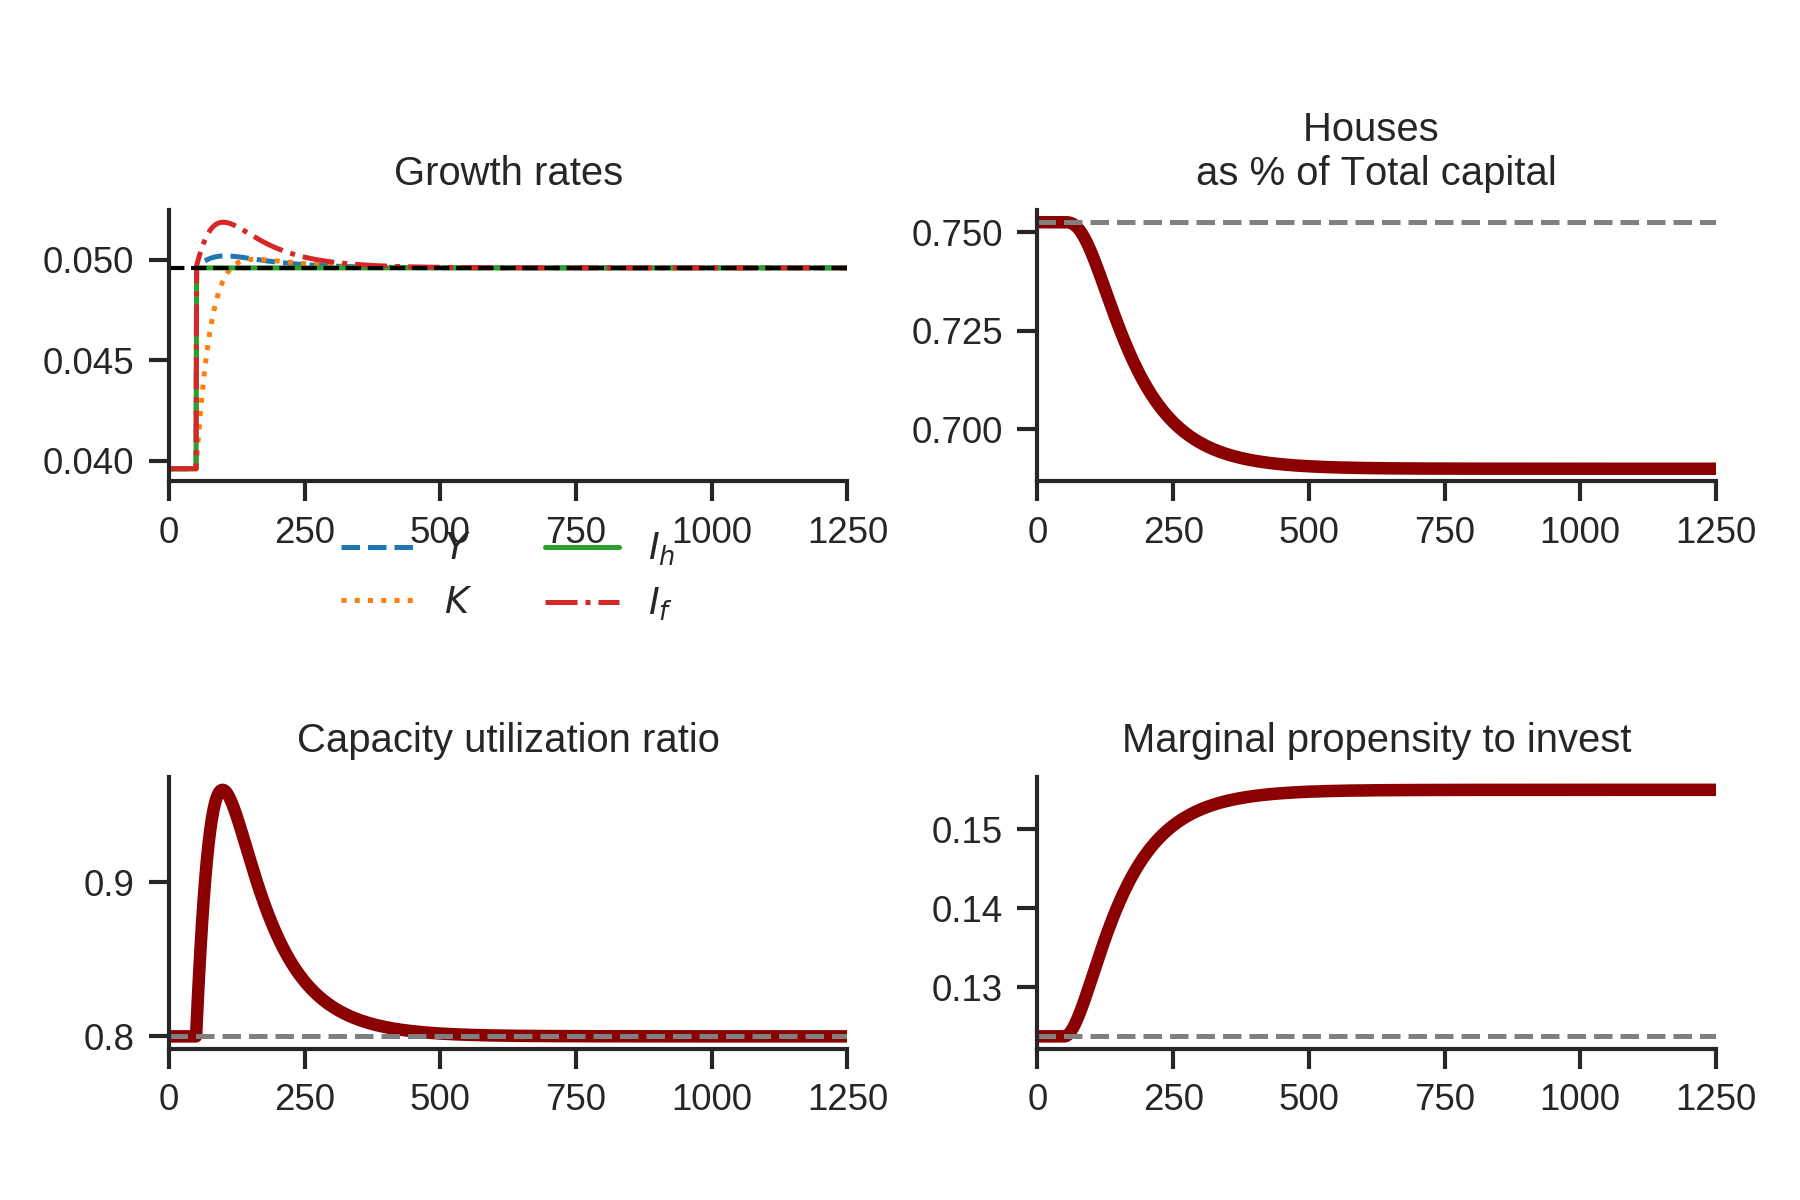
\includegraphics{Modelo/Shock_1.png}
    \caption*{\textbf{Fonte:} Elaboração própria}
\end{figure}


\begin{figure}[htb]
     \centering
     \caption{Resultado dos demais choques}
     \begin{subfigure}[b]{0.45\textwidth}
         \centering
        \caption{Distribuição de renda a favor dos salários}
        \label{choque_2}
        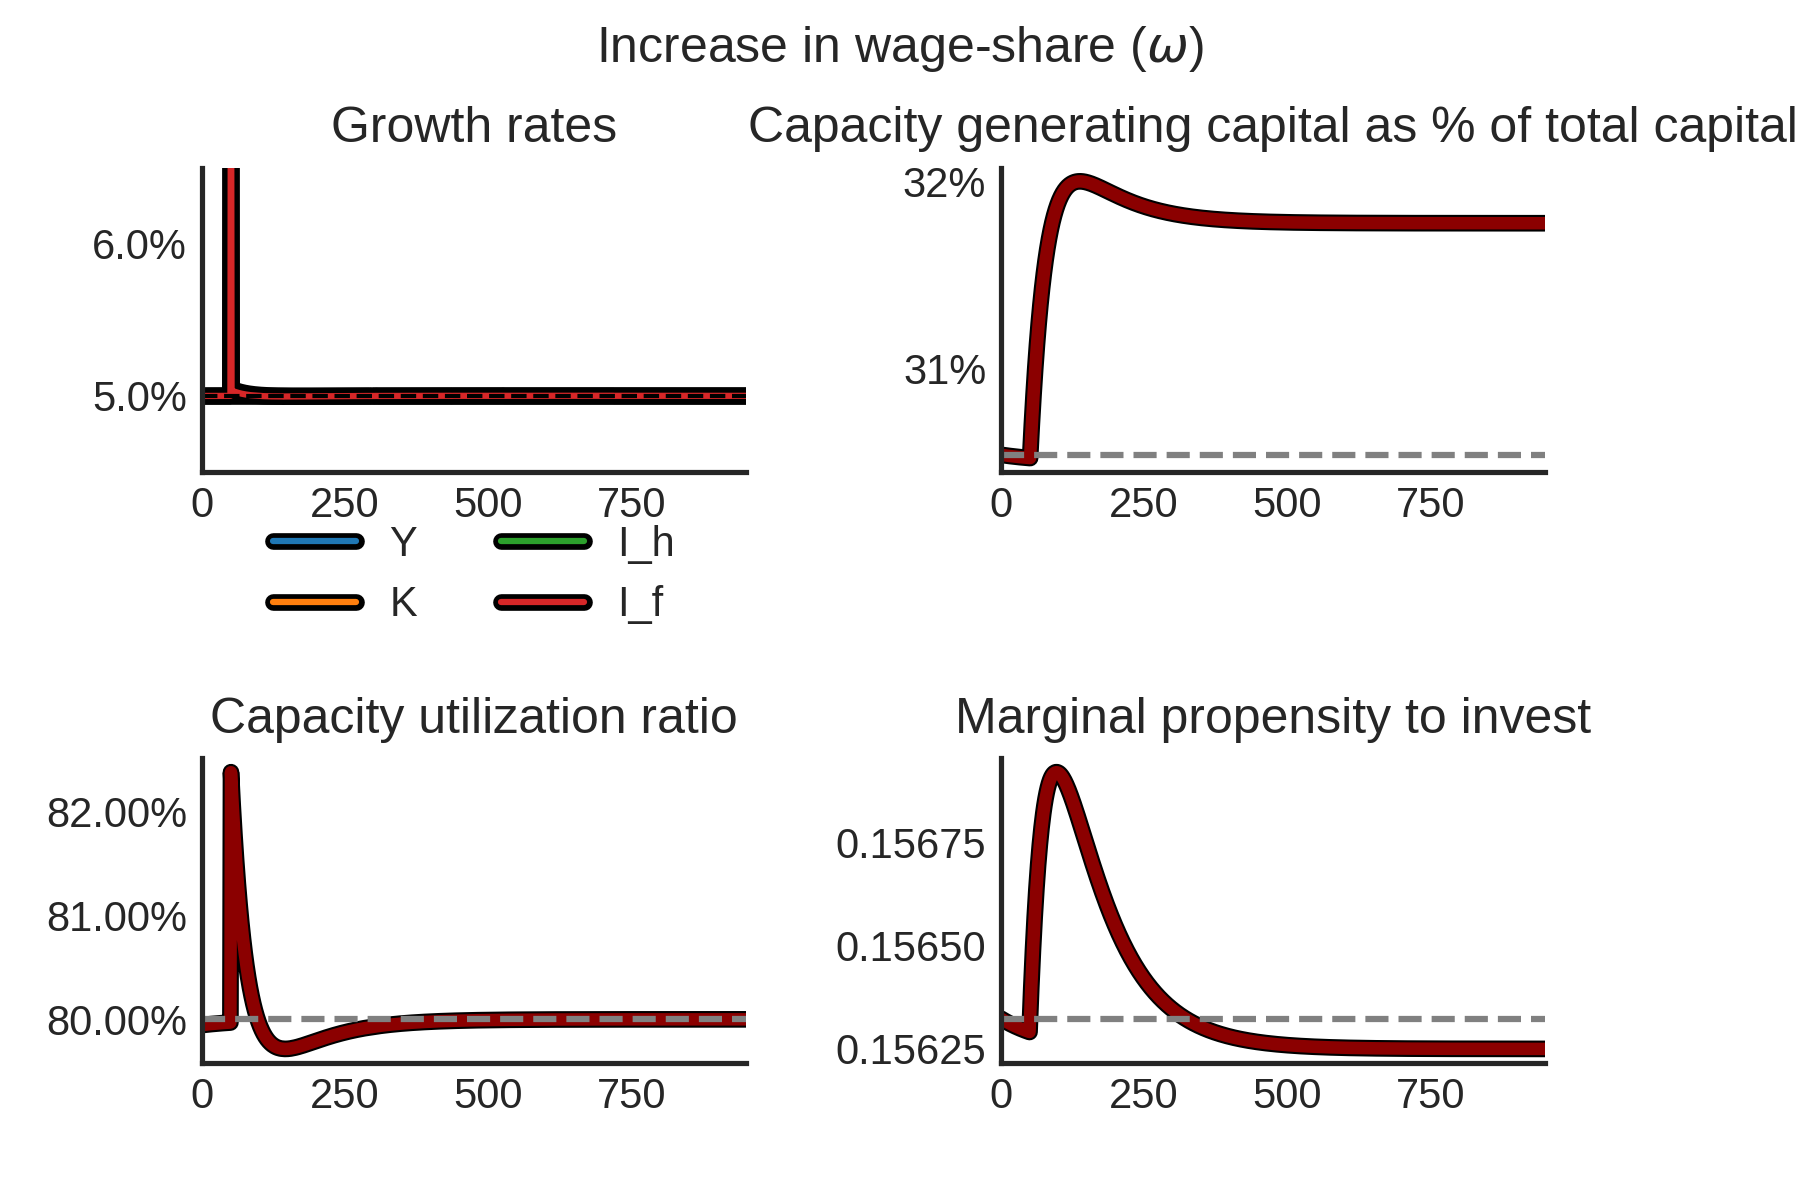
\includegraphics[width = 1\textwidth]{Modelo/Shock_2.png}
     \end{subfigure}
     \hfill
     \begin{subfigure}[b]{0.45\textwidth}
         \centering
         \caption{Aumento na taxa de juros dos depósitos}
         \label{choque_3}
         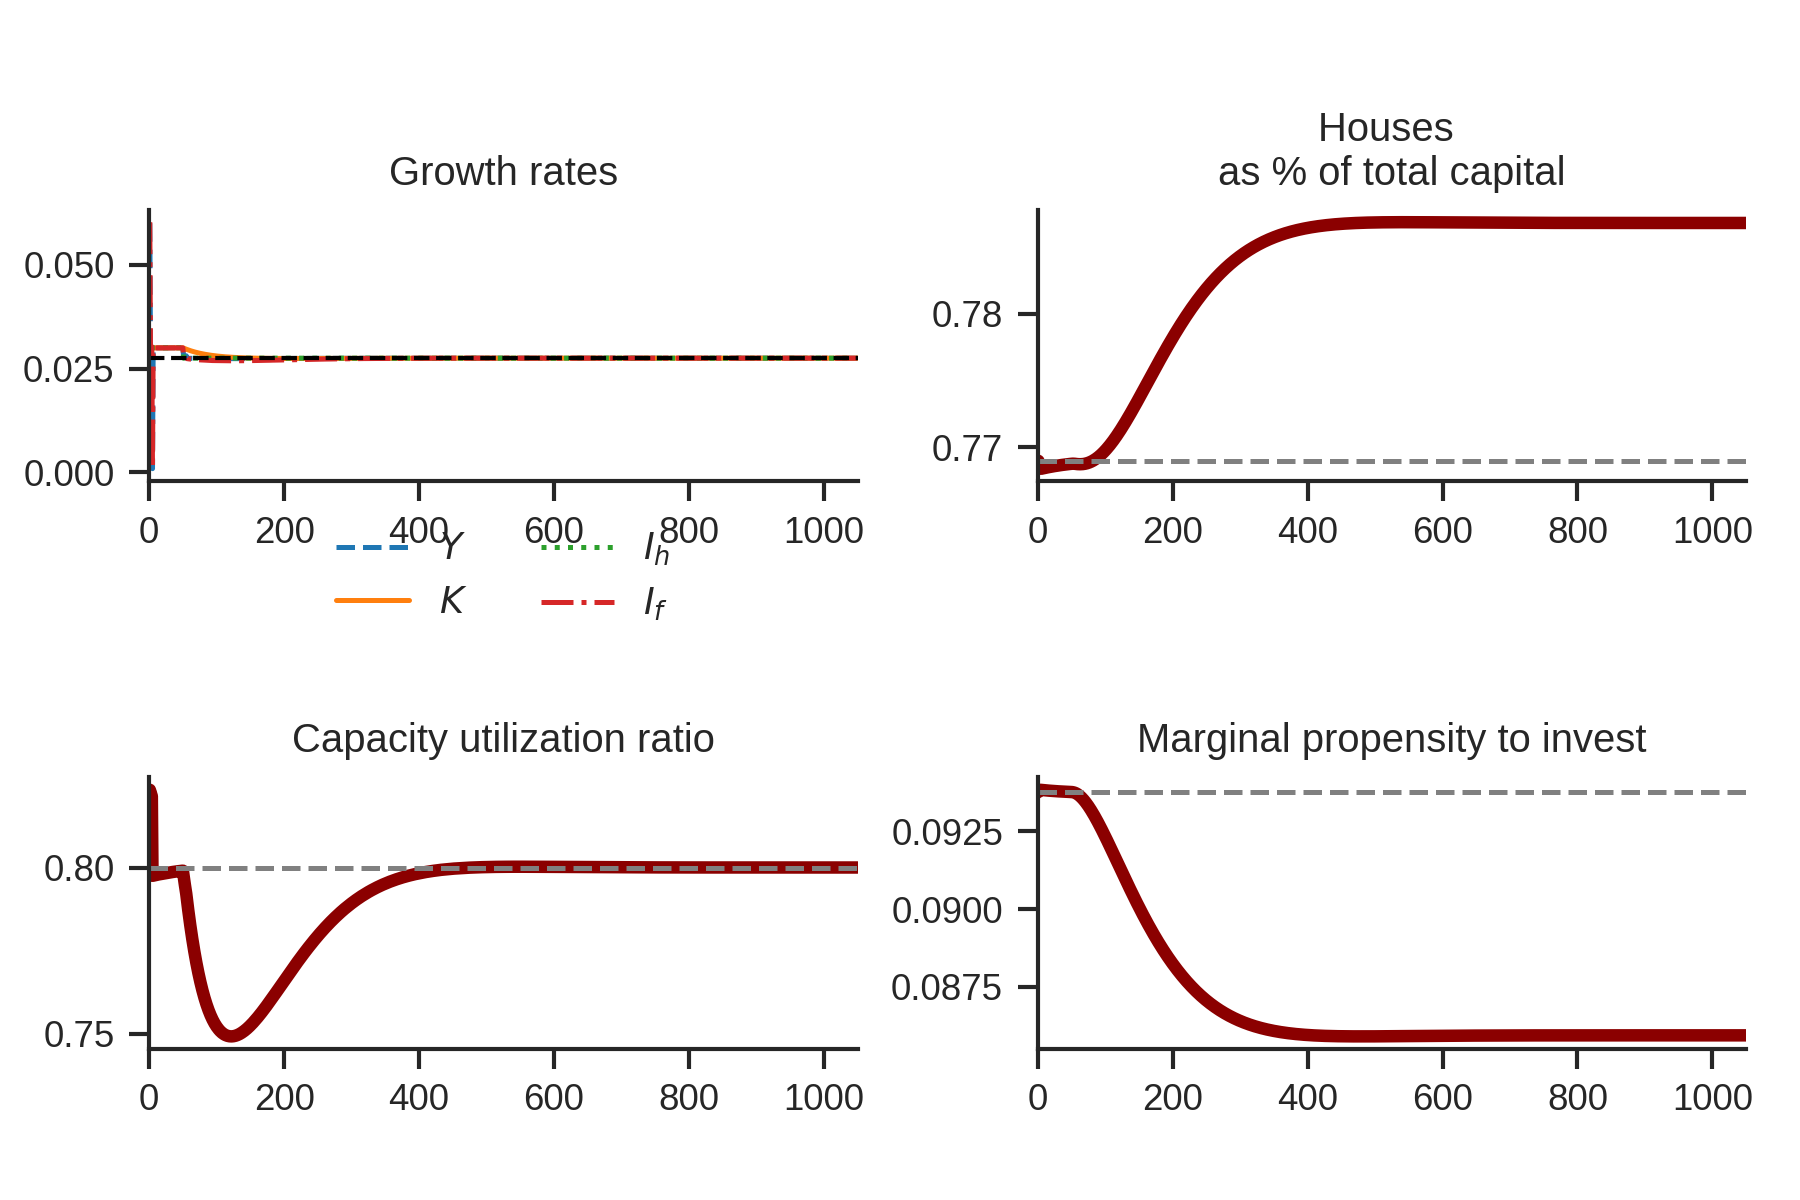
\includegraphics[width = 1\textwidth]{Modelo/Shock_3.png}
     \end{subfigure}
        \caption*{\textbf{Fonte:} Elaboração própria}
        \label{choques}
\end{figure}


\begin{table}[htb]
    \centering
    \caption{Resumo das simulações}
    \label{Resumo_Simulacao}
         \begin{tabular}{ccccc}
\toprule
{} &  Base scenario &  $\Delta g_Z$ &  $\Delta \omega$ &  $\Delta rm$ \\
\midrule
\textbf{$\alpha$    } &          1,000 &         1,000 &            1,000 &        1,000 \\
\textbf{$g_Ih$     } &          0,050 &         0,060 &            0,050 &        0,050 \\
\textbf{$\gamma_F$  } &          0,400 &         0,400 &            0,400 &        0,400 \\
\textbf{$\gamma_u$  }\footnote{Vale mencionar que o valor deste parâmetro é fundamental para garantir a estabilidade do modelo. Os resultados obtidos com as simulações retornaram que valores maiores que 0.07, mantendo os demais parâmetros fixos, impedem que o modelo não colapse.}
                      &          0,010 &         0,010 &            0,010 &        0,010 \\
\textbf{$g_k$       } &          0,050 &         0,060 &            0,050 &        0,050 \\
\textbf{$g_Z$       } &          0,050 &         0,060 &            0,050 &        0,050 \\
\textbf{$h$        } &          0,156 &         0,187 &            0,156 &        0,156 \\
\textbf{$\omega$    } &          0,500 &         0,500 &            0,510 &        0,500 \\
\textbf{$r_l$       } &          0,020 &         0,020 &            0,020 &        0,025 \\
\textbf{$r_m$       } &          0,020 &         0,020 &            0,020 &        0,025 \\
\textbf{$r_{mo}$      } &          0,020 &         0,020 &            0,020 &        0,025 \\
\textbf{$spread_l$ } &          0,000 &         0,000 &            0,000 &        0,000 \\
\textbf{$spread_{mo}$} &          0,000 &         0,000 &            0,000 &        0,000 \\
\textbf{$k$      } &          0,313 &         0,375 &            0,319 &        0,312 \\
\textbf{$u$        } &          0,800 &         0,800 &            0,800 &        0,800 \\
\textbf{$u_N$       } &          0,800 &         0,800 &            0,800 &        0,800 \\
\textbf{$v$        } &          2,500 &         2,500 &            2,500 &        2,500 \\
\bottomrule
\end{tabular}
    \label{Summary_Simplest}
    \caption*{\textbf{Fonte:} Elaboração própria}
\end{table}

\subsection*{Inserindo dados observados: taxa de juros hipotecárias e inflação de imóveis}

Antes de encerrar a discussão do modelo SFC é possível  --- mesmo que de modo preliminar --- avançar em direção a maior aderência ao caso norte-americano recente.
Para tanto, são incluídos dados da taxa própria observados referente ao período do modelo macroeconométrico estimado no capítulo anterior.
Neste ponto, cabe destacar os resultados esperados de acordo com 
alguns dos fatores estilizados reportados no capítulo anterior:
%a literatura do supermultiplicador antes de prosseguir para a inserção dos dados reais:

\begin{enumerate}
\item Relação positiva entre taxa de crescimento e taxa de investimento;
\item Grau de utilização gravita em torno do grau normal apesar de bastante volátil;
\item Aumento do endividamento das famílias associado a redução da renda disponível;
\item Taxas de crescimento acompanham a dinâmica dos gastos autônomos;
%TODO Separar em resultados esperados específicos deste modelo?
\item Investimento residencial é mais volátil que o investimento das firmas e que o produto;
\item Não esgotamento do ajuste da propensão marginal a investir (médio prazo);
%\item Aumento --- seguido de diminuição --- da participação dos imóveis no estoque de capital total da economia.
\end{enumerate}

\begin{figure}[H]
	\centering
	\caption{Taxa de investimento residencial vs Grau de utilização: Inserindo Taxa Própria, taxa de juros hipotecária e inflação de móveis observada}
	\label{clock_Real}
	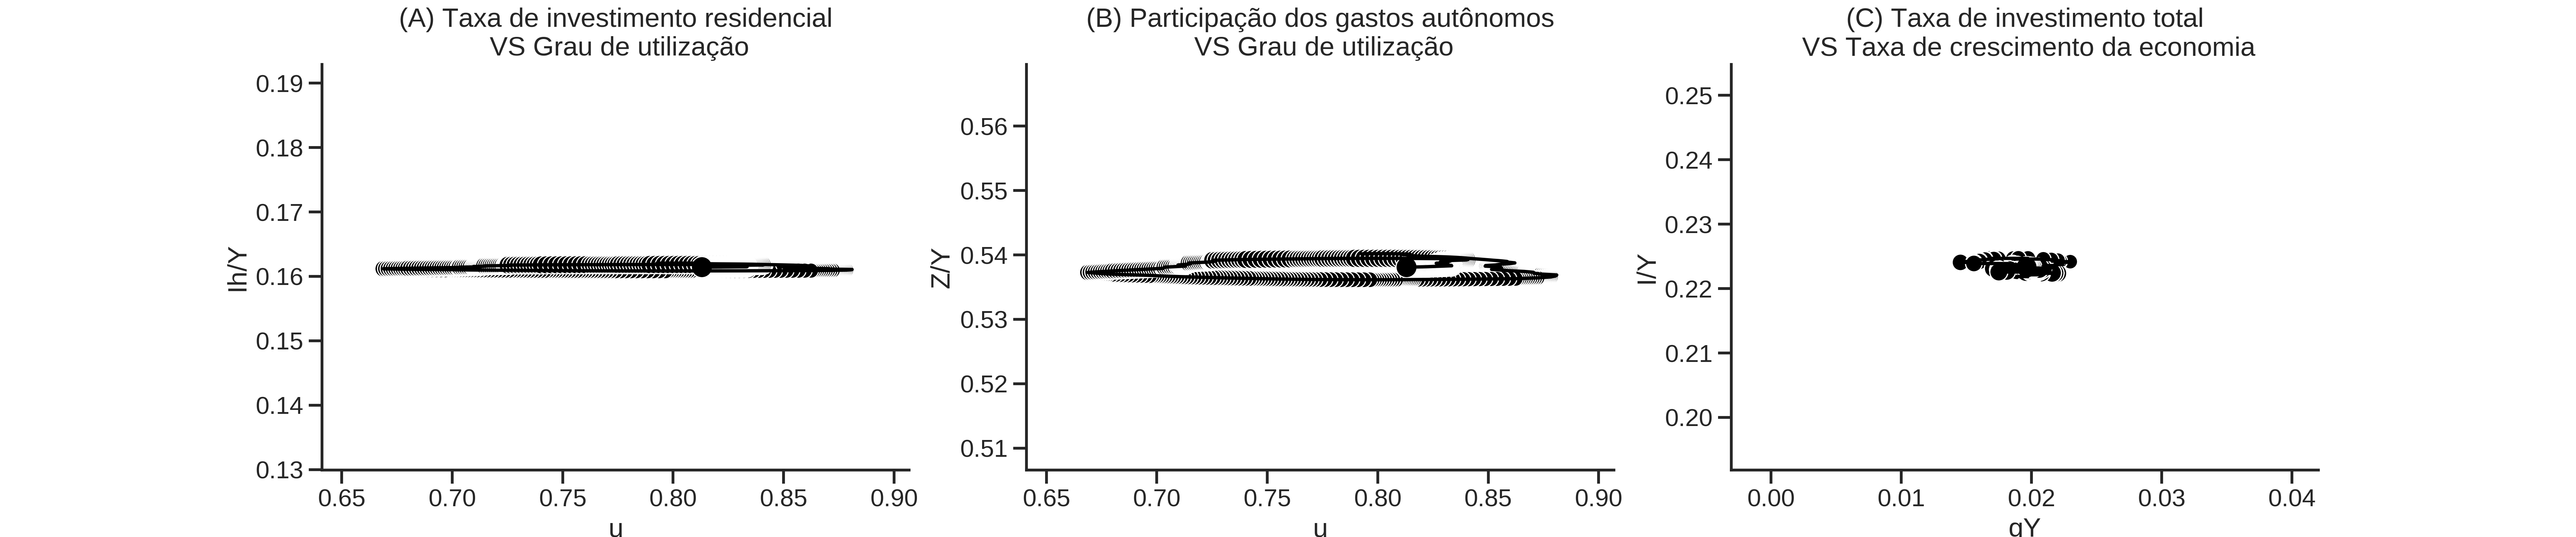
\includegraphics[width=\textwidth]{../../Modelo/Versoes/Clock_Real.png}
	\caption*{\textbf{Fonte:} Elaboração própria}
\end{figure}

Uma primeira aproximação é por meio do gráfico \ref{clock_Real} em que são apresentados --- como no gráfico \ref{FigIh_u} --- e  os gastos autônomos (somente investimento residencial e total) contra grau de utilização, bem como taxa de investimento total (firmas e famílias) e taxa de crescimento da economia.
Uma breve inspeção deste gráfico explicita a relação cíclica e horária entre participação dos gastos autônomos (tanto investimento residencial isolado quanto somado ao crédito aos capitalistas) e nível de atividade tal como discutido no capítulo anterior e o mesmo pode ser dito a respeito da taxa de investimento residencial e grau de utilização. Já o fato estilizado (1) não apresenta um padrão tão demarcado\footnote{A dificuldade de explicitar um padrão bem demarcado também decorre da volatilidade elevada de um dos eixos (taxa de crescimento) enquanto o outro é menos volátil (taxa de investimento).} uma vez que apresenta uma relação positiva entre taxa de investimento e de crescimento em alguns subperíodos e negativa em outros.

\begin{figure}[H]
	\centering
	\caption{Inserindo taxa de juros hipotecária e inflação de móveis observadas}
	\label{choque_Real}
	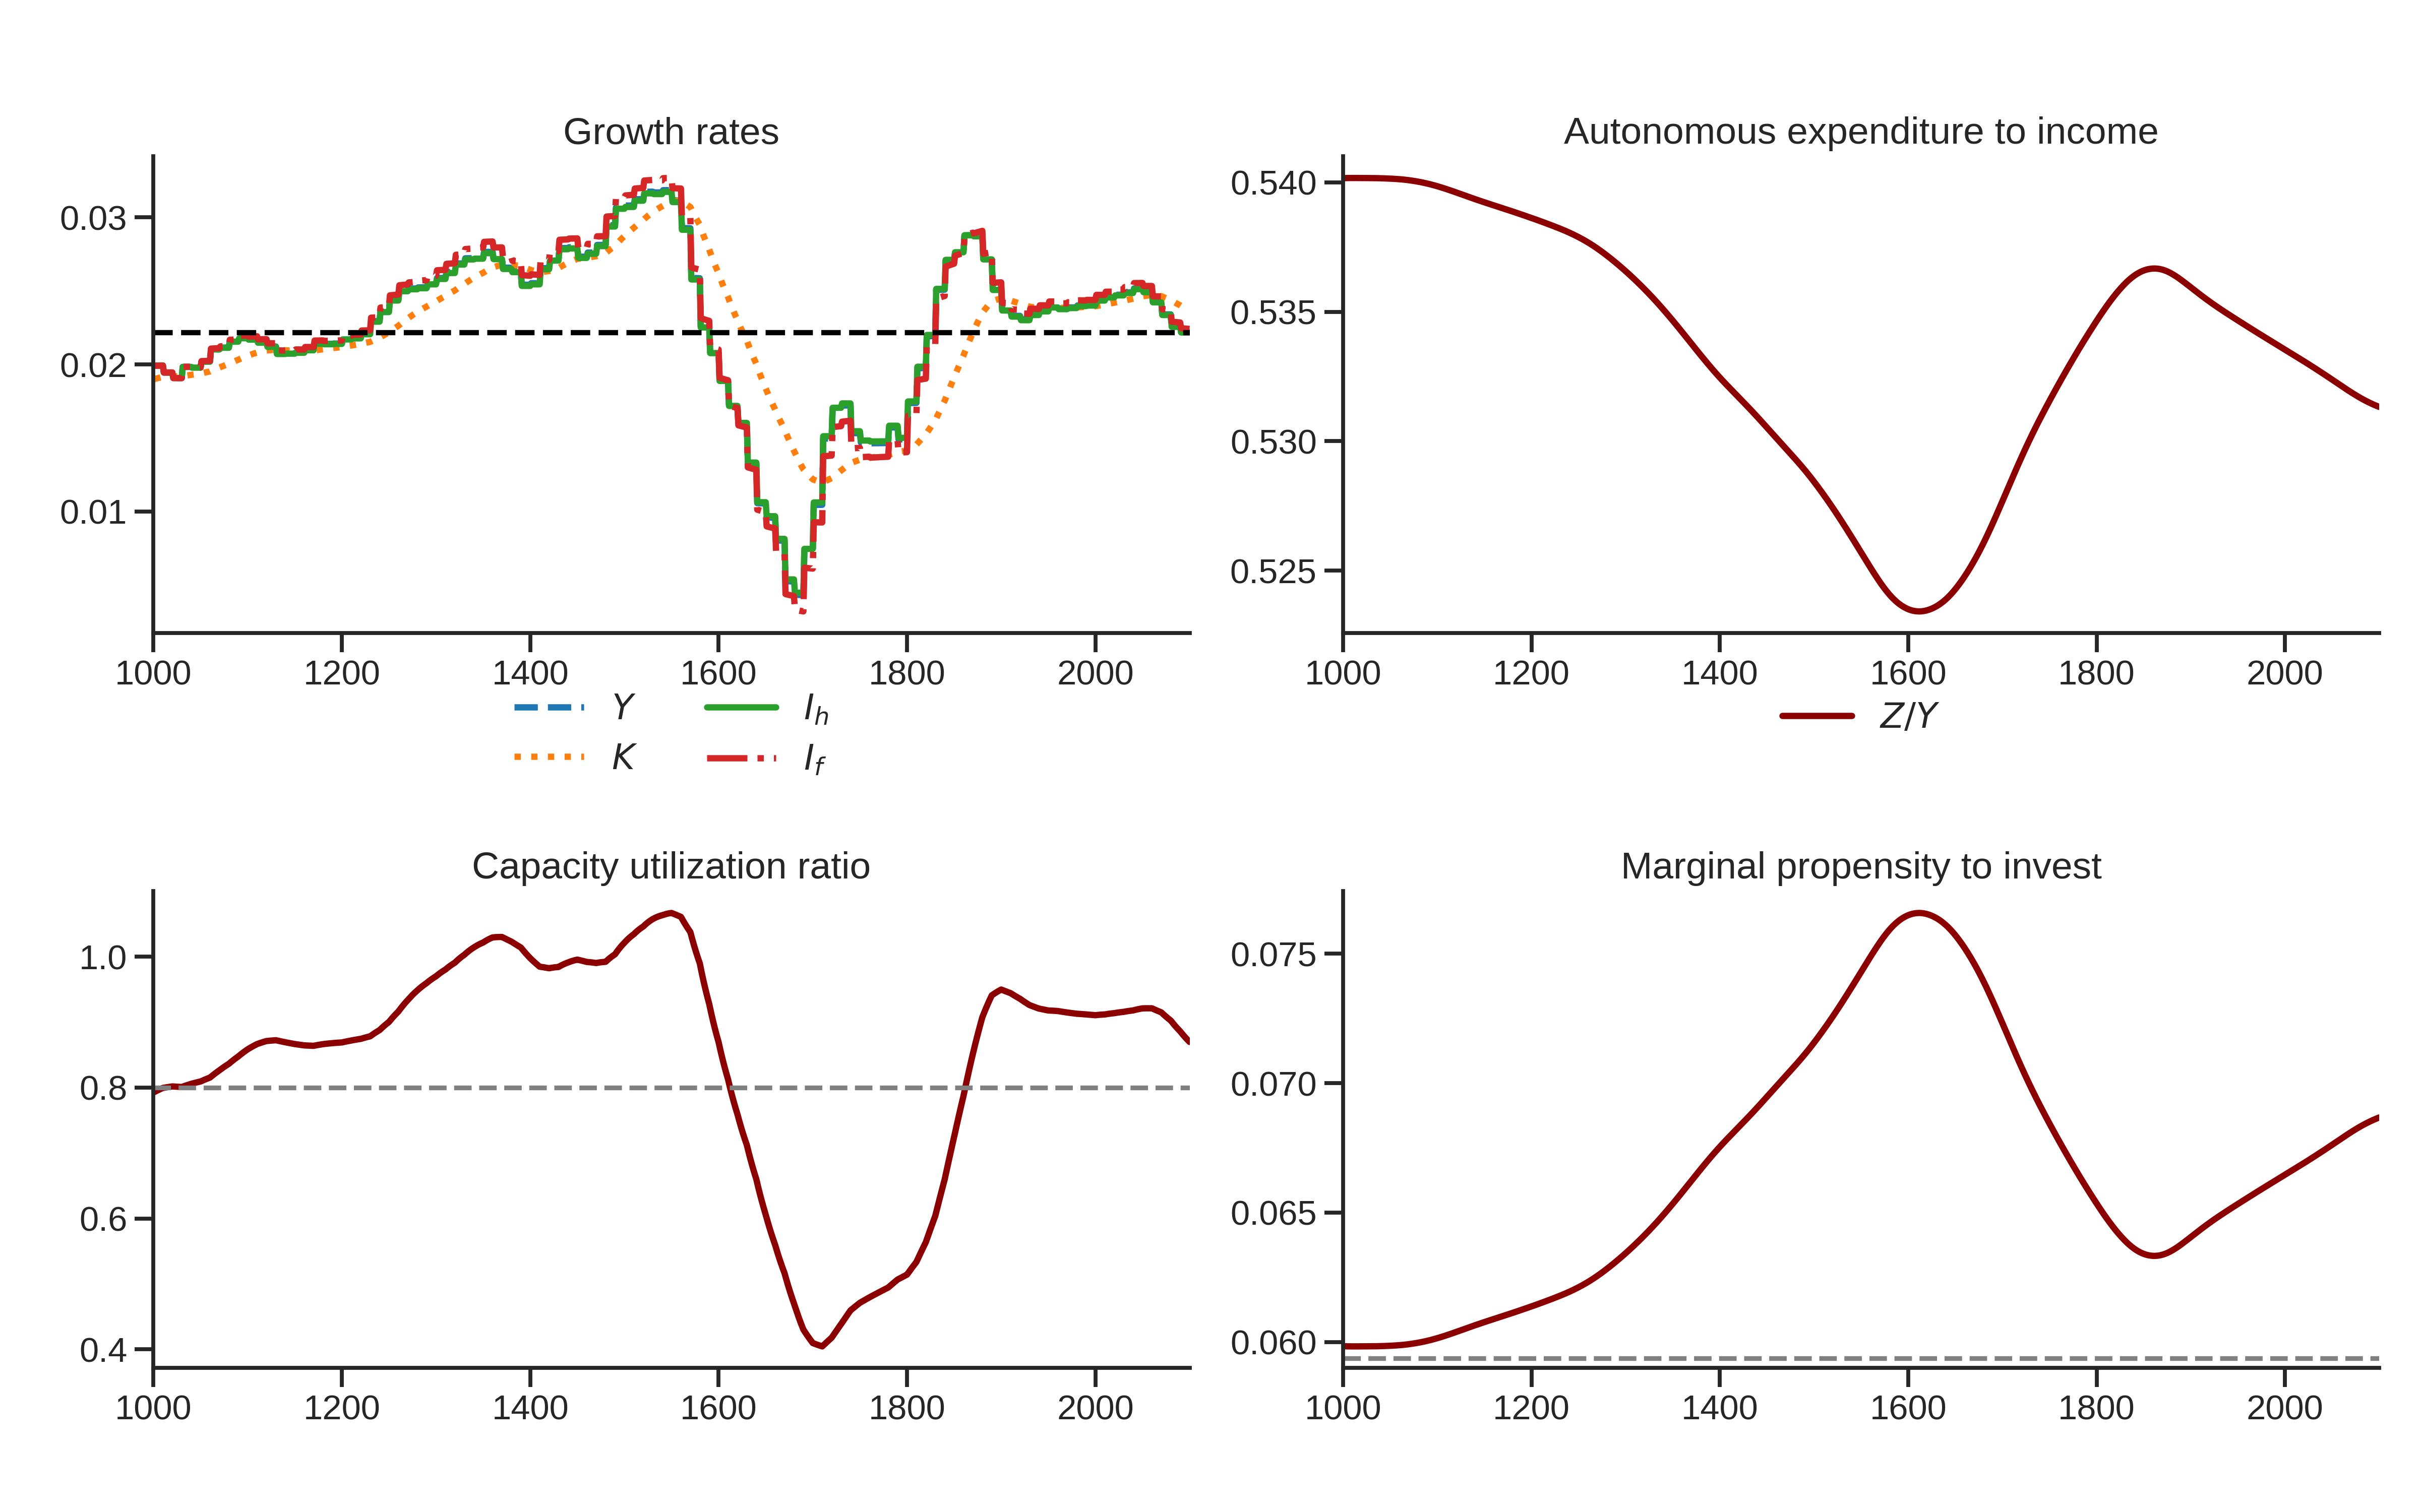
\includegraphics[width=\textwidth]{../../Modelo/Versoes/Shock_Real.png}
	\caption*{\textbf{Fonte:} Elaboração própria}
\end{figure}


O fato estilizado (2) referente ao grau de utilização é contemplado --- feitas as devidas mediações --- uma vez que o período analisado não corresponde a posição plenamente ajustada e, portanto, desvios no grau de utilização em relação ao normal são ajustados por meio de mudanças na propensão marginal a investir (fato estilizado 6). Por fim, destaca-se o acompanhamento da taxa de crescimento da economia aos gastos autônomos, notadamente investimento residencial. No entanto, não é capaz de replicar o fato estilizado (5) de maior volatilidade do investimento residencial.

\begin{figure}[H]
	\centering
	\caption{Inserindo taxa de juros hipotecária e inflação de móveis observadas}
	\label{choque_RealNorms}
	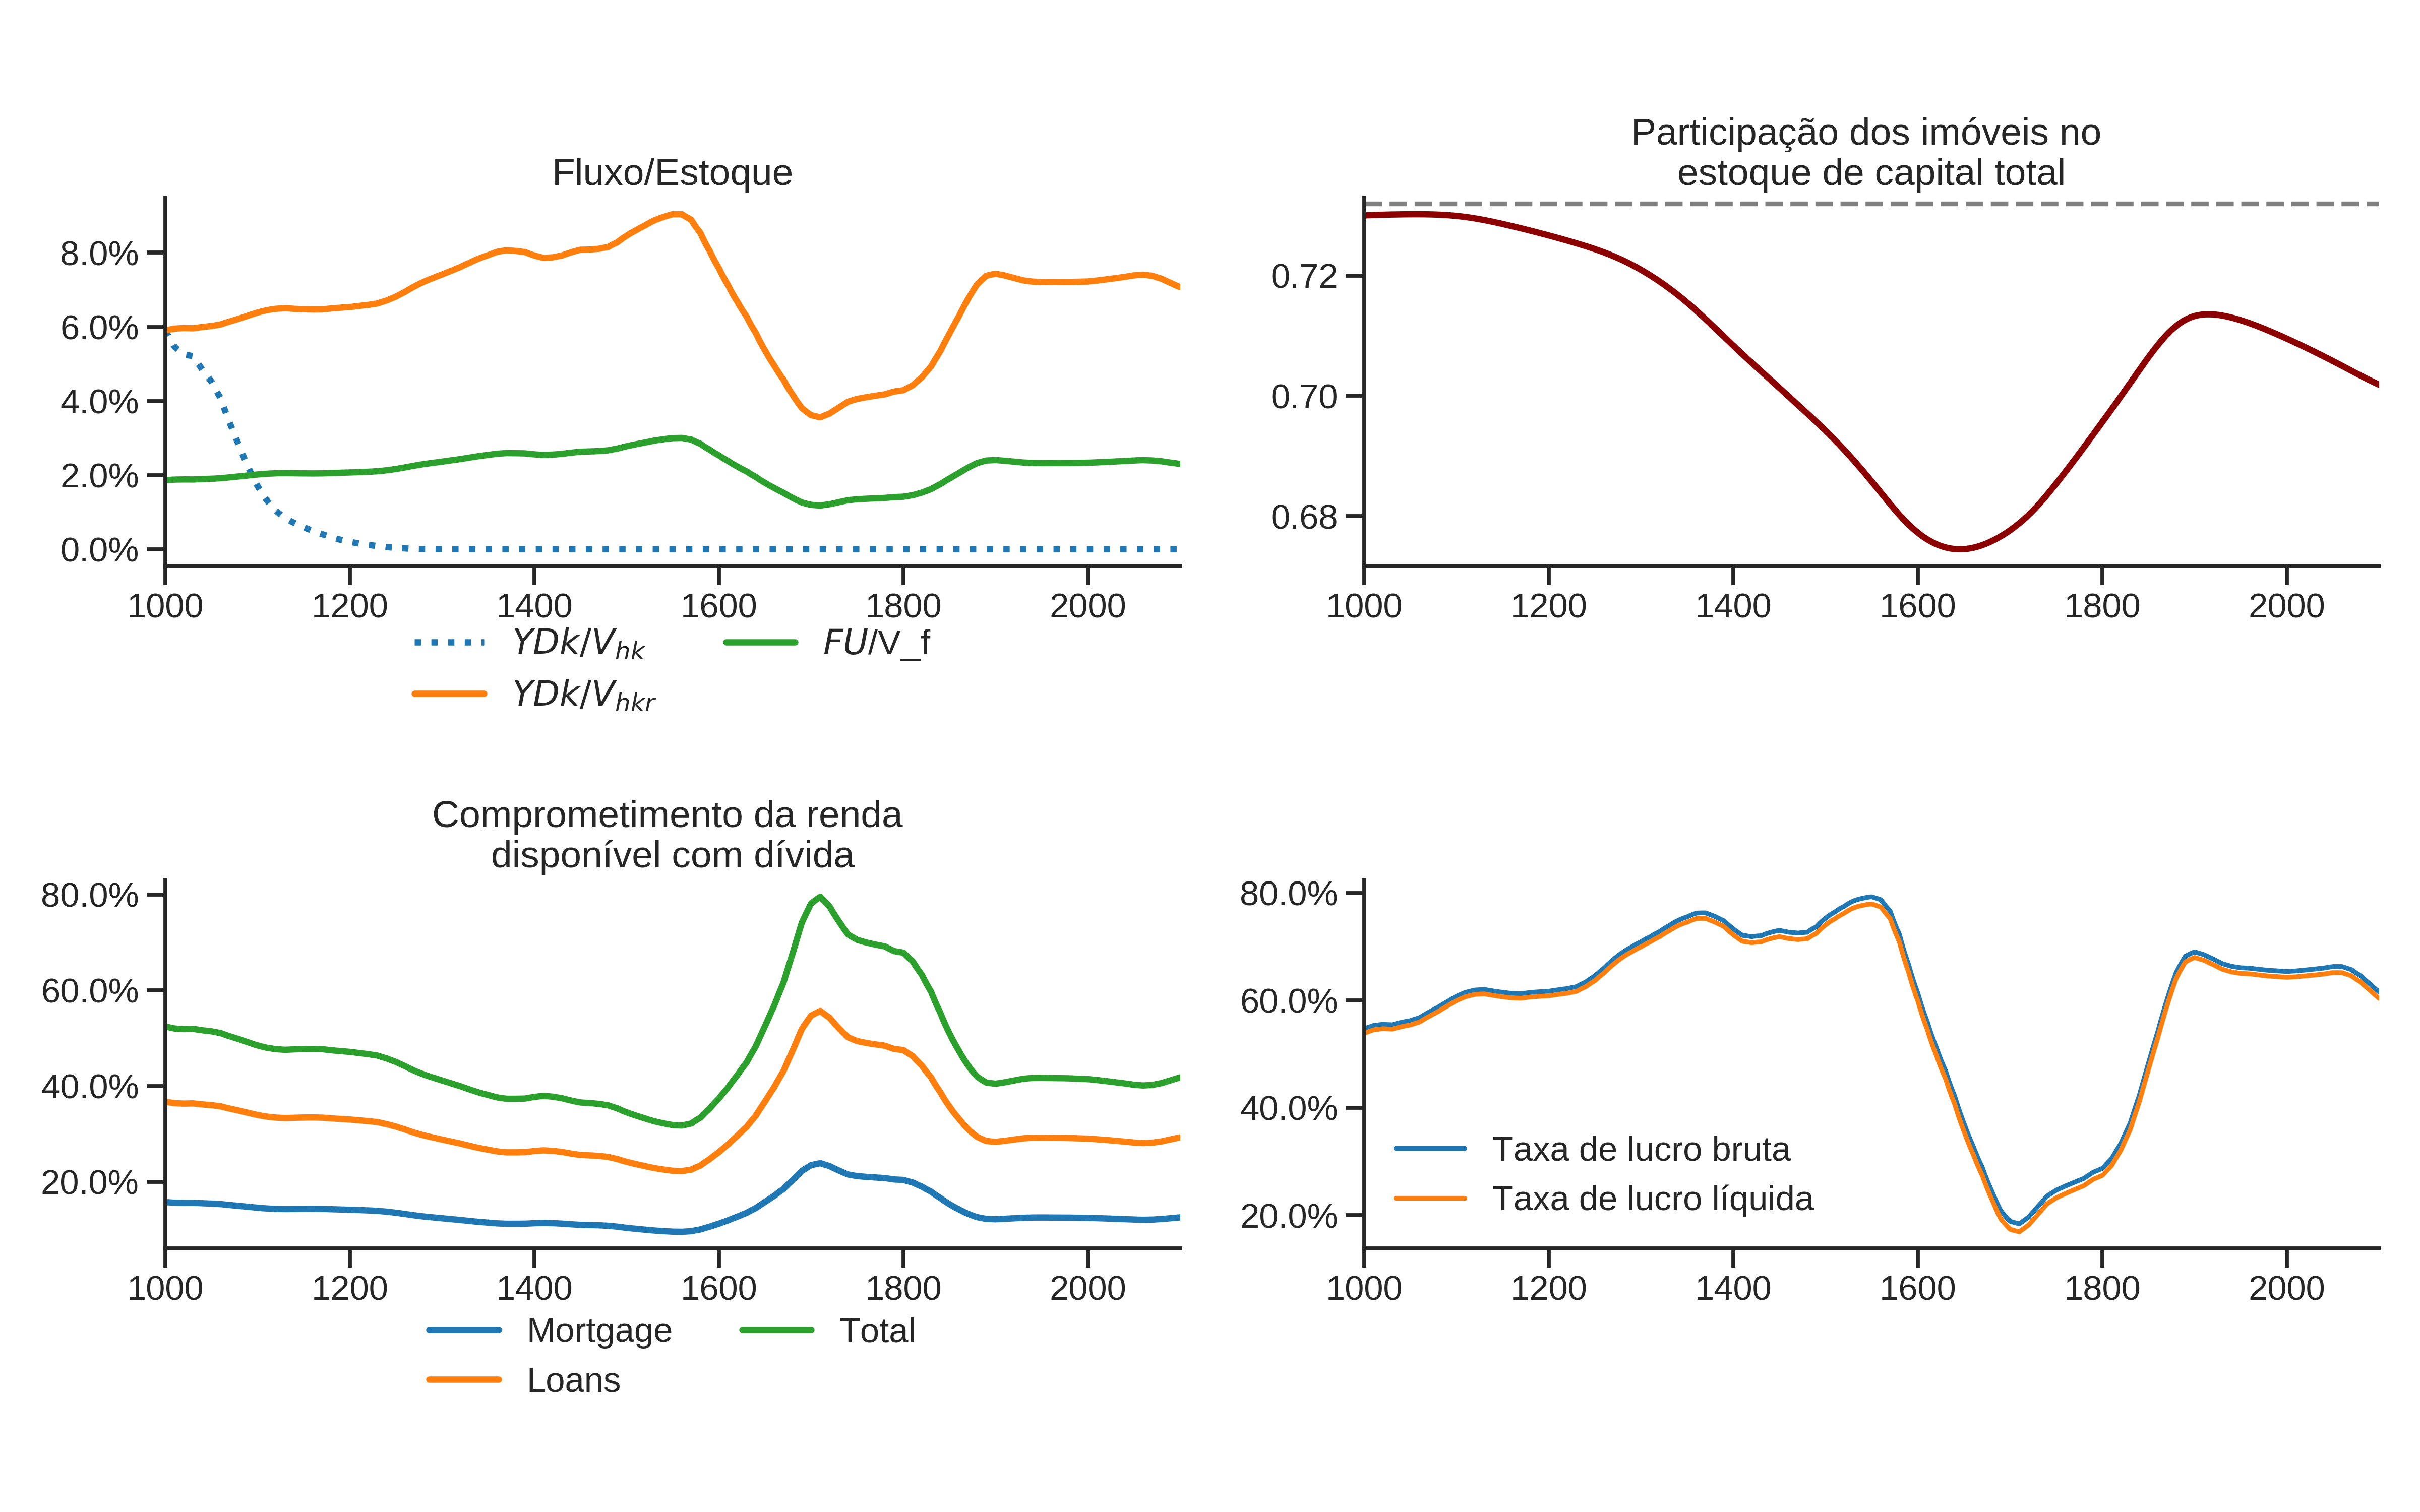
\includegraphics[width=\textwidth]{../../Modelo/Versoes/Shock_RealNorms.png}
	\caption*{\textbf{Fonte:} Elaboração própria}
\end{figure}

Por fim, destaca-se a reprodução do fato estilizado (3) em que tanto o comprometimento da renda das famílias com o pagamento de juros aumenta quanto a razão entre renda disponível em relação a riqueza diminui. Tal dinâmica de endividamento não teve um paralelo nas firmas uma vez que a taxa de lucro bruta e líquida se aproximaram no período equivalente a crise. 
%Além disso, esta simulação reproduz a redução nas taxas de lucro ao longo da crise que está associada a redução do nível de atividade --- dada a participação dos lucros na renda constante.
Vale lembrar que este é um primeiro esforço de confrontar um modelo teórico simulado com investimento residencial frente aos dados observados.
Além disso, tal procedimento não conta com a calibragem dos parâmetros e esta é uma frente de melhoria que versões futuras desta pesquisa pode seguir.
No entanto, os problemas decorrentes desta primeira tentativa de mediação entre teoria e empiria não se restrigem à calibragem. 
Apesar de lançar luz sobre alguns pontos destacados pela teoria, deixa outros em aberto e que devem ser aprimorados preservando as hipóteses do modelo:
\begin{description}
	\item[Temporalidade] Normalmente não é feita uma distinção/discussão nos modelos do tipo SFC de simulação sobre o significado econômico das defasagens adotadas. Sendo assim, para que um modelo teórico tenha maior aderência a empiria é preciso repensar o significado da temporalidade de algumas variáveis;
	\item[Grau de utilização normal] Ao longo desta pesquisa, adotou-se um grau de utilização normal arbitrário (e constante) que, por sua vez, não equivale --- necessariamente --- à média ou à tendência do grau de utilização efetivo. Desse modo, é preciso avançar em direção às formas de incluir tal conceito nos modelos sem que, para isso, seja necessário endogeneizá-lo;
	%incorrer em imprecisões teóricas nem se restringir a arbitrariedade;
	\item[Participação dos gastos autônomos] Tal como o grau de utilização normal, a escolha da participação dos gastos autônomos ($R$) também é arbitrária. Se faz necessário investigar formas de endogeneizar tal participação sem incorrer em soluções assintóticas em que a parcela de um dos gastos convirja a zero;
	\item[Saldo líquido dos setores] Por se tratar de uma economia fechada sem governo, se as famílias forem deficitárias neste modelo as firmas serão necessariamente superavitárias (e o inverso também é válido).
	Sendo assim, para que esta dualidade não seja a única combinação possível se faz necessário incluir outros setores institucionais. No entanto, versões futuras desta pesquisa irão avançar neste nível de complexidade se acrescentar elementos relevantes tanto para a dinâmica do investimento residencial quanto para as implicações macroeconômicas deste gasto. Caso contrário, tais modificações adicionarão complexidade sem incluir --- necessariamente --- maior esclarecimento;
	\item[Composição do patrimônio líquido dos bancos] Ao longo deste capítulo adotou-se a hipótese que os bancos não auferem lucros e, por consequência, não acumulam ativos.
	Sendo assim, tal modelo não consegue reproduzir --- por construção --- razões entre ativos/passivos sobre o patrimônio líquido uma vez que a riqueza (total e financeira) deste setor institucional é nula.
	Desse modo, para que seja capaz de replicar mudanças na composição do patrimônio líquido dos bancos é preciso que este setor passe a obter lucros que, por sua vez, rompe com as hipóteses aqui adotadas.
\end{description}

\section{Considerações finais}\label{Conclusao_Modelo}

Por mais que algumas questões precisam ser melhor desenvolvidas, pontua-se que 
esta pesquisa contribuiu para a literatura de crescimento liderado pela demanda do modelo do supermultiplicador sraffiano, levando em consideração o esforço recente de incorporá-lo em um arcabouço contábil do tipo SFC.  A característica específica do modelo aqui apresentado é a inclusão do investimento residencial. A introdução desse gasto teve como objetivo dar conta dos resultados de alguns trabalhos empíricos recentes que mostram a importância do investimento residencial para dinâmica macroeconômica e, como visto anteriormente, nenhum trabalho havia simulado esse gasto específico via taxa própria de juros dos imóveis. 

O modelo reproduz as principais características do supermultiplicador sraffiano: (i) o grau de utilização converge ao grau normal, por meio de variações da propensão marginal a investir das firmas e; (ii) a taxa de crescimento da economia segue a taxa de crescimento dos gastos autônomos --- nesse caso, o investimento residencial. A primeira diferença do  presente modelo é que o estoque de capital fixo da economia passa a ter dois componentes, o capital produtivo das firmas e os imóveis das famílias. 

Como visto nas simulações, o principal resultado particular deste modelo é que uma maior taxa de crescimento do investimento residencial tem como consequência uma redução da participação do estoque de imóveis no capital total. Tal resultado, aparentemente contra intuitivo, se deve ao ajuste do estoque de capital das firmas. Para que o grau efetivo de utilização da capacidade convirja ao grau normal, o investimento das firmas precisa temporariamente crescer mais rápido que investimento residencial, alterando, portanto, a relação entre os dois estoques. 

Os outros dois experimentos trazem resultados em linha com o supermultiplicador sraffiano. A diminuição da participação dos salários na renda não afeta a taxa de crescimento de longo prazo e, portanto, não afeta a propensão marginal a investir de forma permanente. Porém, por alterar o tamanho do supermultiplicador, diminui a participação do capital produtivo no capital total. O aumento da taxa de juros, por sua vez, tem um efeito tanto sobre a taxa de crescimento de longo prazo quanto sobre o endividamento das famílias em relação à renda disponível. 

É importante destacar que este trabalho é apenas o primeiro passo numa agenda de pesquisa mais ampla sobre o papel do investimento residencial no ciclo e no crescimento econômico. Pesquisas futuras podem (e devem) tornar o modelo aqui apresentado mais complexo. Possíveis extensões incluem explorar outros determinantes do investimento residencial bem como seus impactos sobre outros gastos autônomos e sobre o patrimônio líquido dos bancos.
Com isso, concluí-se os objetivos pretendidos com o modelo apresentado. Cabe ao capítulo seguinte reunir as conclusões desta pesquisa e alguns direcionamentos futuros.

